\subsection{Chapter 14 - Fluid mechanics}

\subsubsection{Overview}\label{chapter:fluidmechanics}

In this chapter, we introduce the tools required to model the dynamics of fluids. This will allow us to model how objects can float, how water flows through a pipe, and how airplane wings create lift. We will start by introducing the concept of pressure and modelling static fluids (hydrostatics) before developing models for fluids that flow (hydrodynamics). Fluids are generally defined as the phase of matter in which atoms (or molecules) are only loosely bound to each other, such as in gases or liquids.  Most of the formalism that we develop will apply to any fluid (gas, liquid, plasma), although we will often restrict ourselves to modelling the most simple situations (e.g. laminar flow of an incompressible liquid).

\begin{framed}
\textbf{Learning Objectives}\\
\begin{itemize}
\item Understand the concept of pressure, and how pressure is modelled in a fluid.
\item Understand how to model the pressure gradient due to gravity.
\item Understand Pascal's Principle and how to model hydraulic lifts and pressure sensing devices.
\item Understand how a pressure gradient leads to a force of buoyancy.
\item Understand the difference between laminar and turbulent flow.
\item Understand the equation of continuity, and the concepts of mass and volumetric flow.
\item Understand how to apply Bernoulli's Principle to model the speed and pressure within a flowing fluid.
\item Understand how to model the resistance to flow in a pipe using the viscosity of a fluid.
\end{itemize}
\end{framed}

\begin{framed}
\textbf{Think About It}\\
You are sailing, and the wind is blowing from the north. You want to travel upwind (north). In what direction should you point your boat/sail?

\begin{figure}[!htbp]
\centering
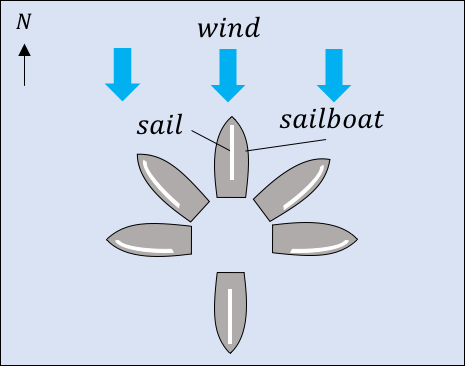
\includegraphics[width=0.4\linewidth]{files/sailboat-73ba0d86d51e365ea42104d9fe2d8ba9.png}
\caption[]{Possible directions you can point your sailboat.}
\label{fig:fluidmechanics:sailboat}
\end{figure}

\begin{enumerate}
\item North
\item South
\item Point either East or West
\item Alternate between North-east and North-west
\item You cannot go upwind.
\end{enumerate}

\begin{framed}
\textbf{Answer}\\
\begin{enumerate}[resume]
\item
\end{enumerate}
\end{framed}
\end{framed}

\subsubsection{Pressure}

The pressure exerted by a force, $\vec F$, over a surface with area, $A$, is a scalar quantity, $P$, defined as:
\begin{equation}
P=\frac{F_\perp}{A}
\end{equation}
where $F_\perp$ is the component of the force perpendicular to the surface. The SI unit for pressure is the Pascal (${\rm Pa}$). Pressure is related to the area, $A$, over which a force is exerted, and can be thought of as a measure of how concentrated that force is. For example, a force of $10 {\rm N}$ exerted through a needle (a small area) will result in a much larger pressure than if that force was exerted by a flat hand (a larger area).

% Pressure is a useful concept for modelling fluids, as the pressure in a fluid can be used to model whether the fluid will move or not.

When a force is exerted on a fluid, it creates pressure that we model as being \textbf{everywhere in the fluid}.
For each element in the fluid, the pressure from the surrounding fluid exerts an inwards force on the element from \textbf{all directions} (see Figure~\ref{fig:fluidmechanics:pressure}). In reaction, the element exerts an outwards force in all directions, and these forces act on neighbouring elements.

This is somewhat analogous to the tension that exists everywhere in a rope, where each element of the rope experiences forces from the neighbouring elements in rope that try to ``pull it apart''. Pressure can be thought of as a ``negative'' tension, in that the material under pressure is experiencing forces trying to collapse the element onto itself, rather than trying to pull it apart. To create a tension in a rope, one would exert an outwards force on the rope (in order to stretch it), so that the rope exerts an inwards force in reaction. In order to create pressure in a fluid, one must exert an inwards force on the fluid, which then exerts an outwards force in reaction.

If we consider a small cubic volume of fluid, as depicted in the centre of Figure~\ref{fig:fluidmechanics:pressure}, that element of fluid will experience inwards forces in all directions from the pressure in the surrounding fluid, as illustrated by the arrows. If the forces from the pressure result in no net force on the fluid element, then we say that the fluid is in hydrostatic equilibrium, and the element of fluid will be at rest in an inertial frame of reference.

\begin{figure}[!htbp]
\centering
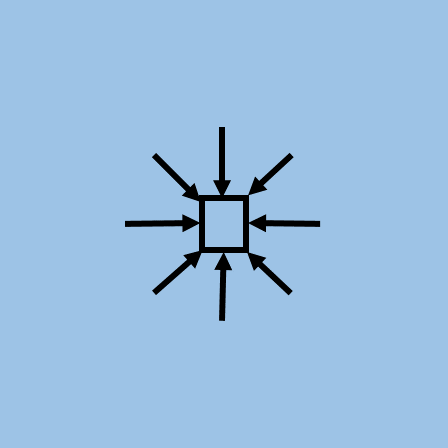
\includegraphics[width=0.4\linewidth]{files/pressure-5816848d52c5e9d5fb3b5be554244cb1.png}
\caption[]{A small element inside of a fluid with pressure will experience no net force from the pressure in the fluid, since the force associated with the pressure in the fluid is exerted in all directions.}
\label{fig:fluidmechanics:pressure}
\end{figure}

Consider, instead, an element of fluid that at the edge of a container for the fluid (e.g. a cup of water), as depicted in Figure~\ref{fig:fluidmechanics:pressure_edge}.

\begin{figure}[!htbp]
\centering
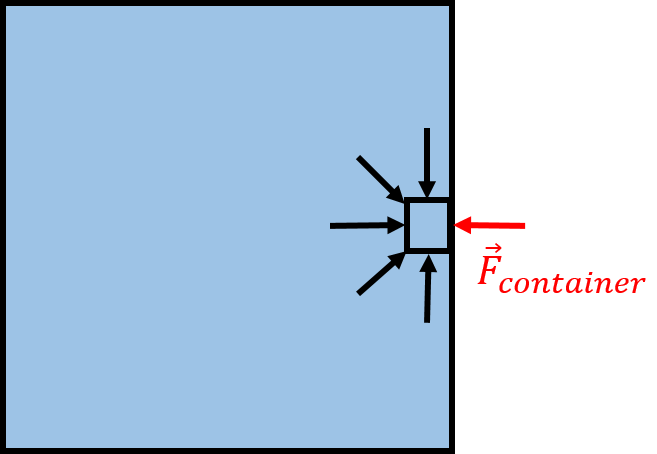
\includegraphics[width=0.5\linewidth]{files/pressure_edge-c7179da01e0197a8960032a3a1a63f11.png}
\caption[]{At the edge of a container, a small element of fluid will exert an outwards force on the container, and the container will exert an inwards force on the element of fluid.}
\label{fig:fluidmechanics:pressure_edge}
\end{figure}

In this case, there is no fluid on the right-hand side of the fluid element to exert a force towards the left. If the fluid element is in equilibrium, it must then be the container that exerts that force, $\vec F_{container}$, on the fluid. By Newton's Third Law, the element of fluid exerts an outwards force on the container. This is true at all points on the surface of container, which will all experience an outwards force from the pressure of the fluid. If the pressure is constant over a surface, the magnitude of the outwards force on the surface will be equal to the pressure of the fluid multiplied by the area of that surface.

If you place an empty sealed tin can under water, the water will exert a pressure on all of the surfaces of the tin can that leads to a net inwards force on all surfaces of the tin can. If the water pressure is high enough, the tin can will get crushed. If, on the other hand, the tin can is allowed to fill with water, it will not get crushed, as the water inside the tin can will have the same pressure as the water outside the tin can and will exert an equal net outwards force on all surfaces of the tin can. The net force on each surface of the can will be zero, and the tin can will not get crushed, no matter how high the water pressure is.

In general, if there is an interface with fluid on either side of it a different pressures, it is the \textbf{difference in pressure} on either side of the interface that determines the net force exerted on the interface, rather than the absolute pressure.

\begin{framed}
\textbf{Checkpoint}\\
You place a tin can on a table, and use a pump to create a vacuum inside of the can. You observe that the tin can gets crushed. Which explanation is correct?

\begin{enumerate}
\item By sucking the air out of the can, you also suck in on the walls of the can.
\item You lower the pressure inside the can so that the air outside the can exerts a larger inwards force on the can than the outwards force from the air inside the can.
\item You lower the pressure inside the can so that the air inside the can exerts a pulling force on the walls of the can.
\item All of the above are all valid ways to model this.
\end{enumerate}

\begin{framed}
\textbf{Answer}\\
\begin{enumerate}[resume]
\item
\end{enumerate}
\end{framed}
\end{framed}

\paragraph{The effect of gravity}

When discussing Figure~\ref{fig:fluidmechanics:pressure}, we argued that the fluid exerts an equal force, from all directions, on the fluid element, so that the net force on the fluid element is zero. This is not quite correct in the presence of gravity, where the fluid element will have a weight. Thus, if the fluid element is to be in equilibrium, the upwards force (and pressure) from the fluid below must be higher than that from the fluid above the fluid element.

Figure~\ref{fig:fluidmechanics:pressure_gravity} shows an element of fluid that has a height $h$ and a surface area $A$ in the horizontal plane. The pressure, $P_2$, in the fluid below the fluid element must be higher than the pressure, $P_1$, above the fluid element, if the fluid element is in equilibrium.

\begin{figure}[!htbp]
\centering
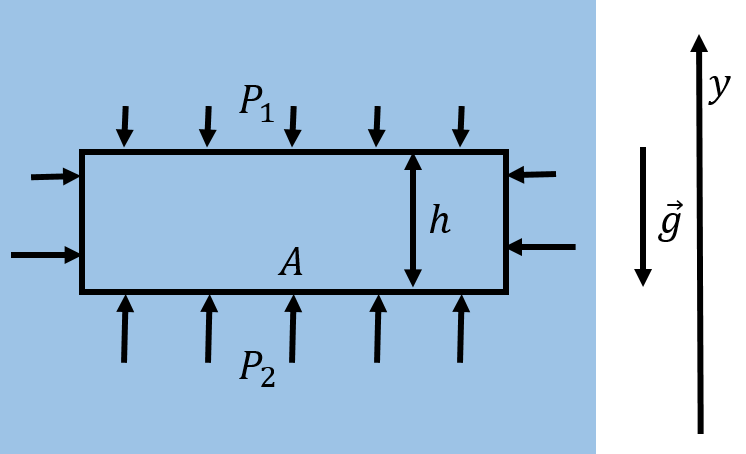
\includegraphics[width=0.5\linewidth]{files/pressure_gravity-59c4653e474bbfdc4fc02ca8428ba1d9.png}
\caption[]{In the presence of gravity, the pressure below an element of fluid must be larger if the fluid element is to remain in equilibrium.}
\label{fig:fluidmechanics:pressure_gravity}
\end{figure}

The element of fluid has a total mass, $m$, given by:
\begin{equation}
m = \rho V = \rho Ah
\end{equation}
where, $V=Ah$, is the volume of the fluid, and, $\rho$, its density.

The net (horizontal) force exerted by the external fluid on the fluid element is zero along the vertical surfaces. Let $P_1$ be the pressure in the fluid above the fluid element, and $P_2$ be the pressure below the fluid element. If we choose a $y$ axis that is positive upwards and the fluid element does not accelerate in the vertical direction, then the $y$ component of Newton's Second Law, written for the fluid element, is:
\begin{equation}
\sum F_y = F_2 - F_1 -mg &= 0\\
P_2A - P_1A-mg &=0\\
P_2A - P_1A-\rho Ahg &=0\\
\therefore P_2 - P_1 = \rho gh
\end{equation}
where we used the fact that the force resulting from a pressure is given by the pressure multiplied by the area over which it is exerted. We thus find that the difference in pressure due to gravity in a fluid between two positions, $y_2$ and $y_1$, is given by:
\begin{equation}
\label{eq:fluidmechanics:pgrav}
\boxed{P(y_2) - P(y_1) = -\rho g (y_2 - y_1)}
\end{equation}
where the $y$ axis is defined to increase in the upwards direction. Since the pressure in the fluid depends on the location in the fluid, we say that there is a ``pressure gradient'' in the fluid.

\begin{framed}
\textbf{Checkpoint}\\
\begin{figure}[!htbp]
\centering
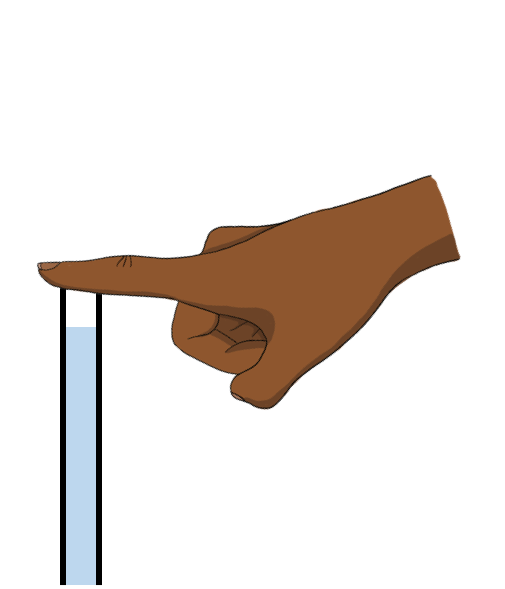
\includegraphics[width=0.3\linewidth]{files/straw-0483ee878cc7e8253673516294129401.png}
\caption[]{Holding water in a vertical straw.}
\label{fig:fluidmechanics:straw}
\end{figure}

You use your finger to block off the top end of a straw and then remove the straw from a glass of water. What is the most correct description of why the water stays in the straw (Figure~\ref{fig:fluidmechanics:straw}) before you release your finger?

\begin{enumerate}
\item The straw cannot have vacuum inside of it; unless the finger is removed to let air in to replace the water, the water will remain in the straw.
\item There is a small amount of vacuum above the water that sucks the water upwards and prevents it from dropping.
\item The pressure of the air in the straw below the water is higher than the pressure of the air in the straw above the water.
\item The pressure of the air in the straw below the water is lower than the pressure of the air in the straw above the water.
\end{enumerate}

\begin{framed}
\textbf{Answer}\\
\begin{enumerate}[resume]
\item
\end{enumerate}
\end{framed}
\end{framed}

We have assumed that the density of the fluid, $\rho$, is constant, and that the fluid cannot be compressed. This is a very good approximation for a liquid such as water, but not for a gas, whose density will depend on its pressure. If the fluid were a gas (e.g. a column of air in our atmosphere), both the density and the pressure will change as a function of height. We can easily take this into account in our model, if we consider the fluid element to have a very small height, $dy$, instead of the finite height, $h$, as in the derivation above. A fluid element with an infinitesimal height, $dy$, is illustrated in Figure~\ref{fig:fluidmechanics:pressure_gravity2}.

\begin{figure}[!htbp]
\centering
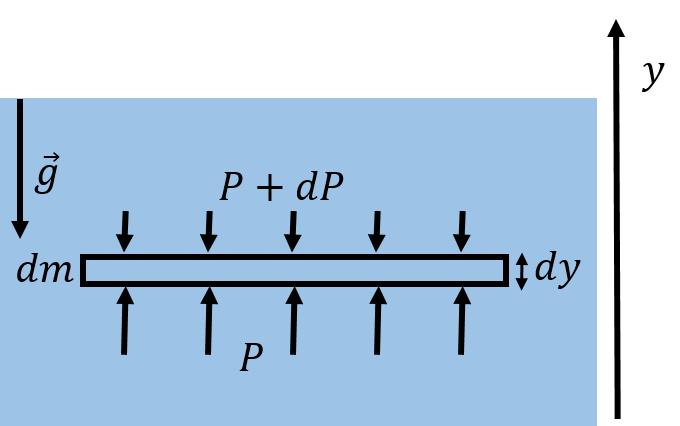
\includegraphics[width=0.4\linewidth]{files/pressure_gravity2-d4fd6b679d8097440487920fb60efc66.png}
\caption[]{Pressure gradient from gravity on an infinitesimal fluid element.}
\label{fig:fluidmechanics:pressure_gravity2}
\end{figure}

In the very small height, $dy$, the density of the fluid, $\rho$, can be taken to be constant, and the infinitesimal element of fluid will have a mass $dm$:
\begin{equation}
dm = \rho A dy
\end{equation}
We can model the pressure exerted by the fluid above the fluid element as $P+dP$, and the pressure exerted by the fluid below as $P$, where $dP$ is a small (negative) change in pressure\footnote{We placed the $dP$ on the top part of the fluid, even though the pressure is higher on the bottom part of the fluid, because the $y$ axis increases upwards. We are really interested in the change in pressure, $dP$, that corresponds to a change in height, $dy$, along the positive $y$ direction.}. The $y$ component of Newton's Second Law written for the infinitesimal fluid element is thus:
\begin{equation}
\sum F_y = PA - (P+dP)A -dm g &=0\\
PA -PA -dPA - \rho A dy g &=0\\
\therefore -dP -\rho gdy &=0
\end{equation}
We can thus determine how pressure changes with height, $y$:
\begin{equation}
\boxed{\frac{dP}{dy} = -\rho g}
\end{equation}
This tells us that the rate of change of pressure with increasing $y$ is negative; in other words, the pressure decreases as the elevation increases, as we had already concluded. We can integrate the equation to obtain the change in pressure in going from $y_1$ to $y_2$:
\begin{equation}
dP &= -\rho g dy\\
\int_{P_1}^{P_2} dp&=-\int_{y_1}^{y_2}\rho gdy\\
\therefore P_2-P_1 &=-\int_{y_1}^{y_2}\rho gdy
\end{equation}
If the density, $\rho$, is constant, then this leads to (\ref{eq:fluidmechanics:pgrav}). Note that, thus far, we have only modelled how pressure in a fluid changes with height, but we have not determined the absolute pressure in a fluid.

\begin{framed}
\textbf{Example 14.1}\\
If we assume that the density of air is proportional to its pressure, how does the density of air change with altitude?

\begin{framed}
\textbf{Solution}\\
We know that the rate of change of pressure with altitude (position $y$, where positive $y$ is defined to be upwards) is given by:
\begin{equation}
\frac{dP}{dy} &= -\rho g
\end{equation}
Since we can assume that the density is proportional to the pressure, we can introduce an arbitrary constant, $a$, and state that:
\begin{equation}
\rho &=aP\\
\therefore \frac{dP}{dy} &=  \frac{d}{dy} \frac{1}{a} \rho = \frac{1}{a}  \frac{d\rho}{dy}
\end{equation}
where the constant $a$ can be evaluated if we know the pressure and density at some point. We can thus write that the rate of change of the density with position $y$ is given by:
\begin{equation}
 \frac{1}{a} \frac{d\rho}{dy} &= -\rho g\\
 \therefore \frac{d\rho}{dy} &= -ag \rho
\end{equation}
This is a separable differential equation for $\rho$, allowing us to separate the variables and integrate from, say, an altitude of $y=0$, where the density is $\rho_0$, to an altitude $y$, where the density is $\rho$:
\begin{equation}
\frac{d\rho}{\rho} &= - ag dy\\
\int_{\rho_0}^{\rho}\frac{d\rho}{\rho} &= -\int_{0}^{y}agdy\\
\ln(\rho)-\ln(\rho_0)&= -agy\\
\ln\left( \frac{\rho}{\rho_0} \right)&= -agy
\end{equation}
We can take the exponential on each side of the equation to get rid of the logarithm:
\begin{equation}
\frac{\rho}{\rho_0} &= e^{-agy}\\
\therefore \rho(y) &= \rho_0e^{-agy}
\end{equation}
We thus find that the density of the air decreases exponentially with altitude. This is why it is more difficult to breathe at high altitude. Since we assumed that the density of the air is proportional to its pressure, the air pressure will also decrease exponentially with increasing altitude:
\begin{equation}
P(y) &= P_0e^{-agy}
\end{equation}
where $P_0$ is the pressure at an altitude of $y=0$. If we know $P_0$ and $\rho_0$, then the constant $a$ is given by:
\begin{equation}
a = \frac{\rho_0}{P_0}
\end{equation}

\textbf{Discussion:} If we applied this model to the Earth's atmosphere, our model would only provide qualitative agreement, as the density of the air also depends on its temperature and other factors. Nonetheless, it is interesting that, based on the simple requirement that an element of air be in hydrostatic equilibrium, we are able to obtain a reasonable description of how pressure and density change with altitude in the Earth's atmosphere.
\end{framed}
\end{framed}

\paragraph{Pascal's Principle}

Pascal's Principle states that \textbf{if an external pressure is exerted on a fluid, the pressure everywhere in the fluid increases by that amount}. For example, if a fluid is contained in a piston with a cross-section area, $A$, and a force, $F$, is exerted on the piston (Figure~\ref{fig:fluidmechanics:piston}), then the pressure everywhere in the fluid increase by $F/A$.

\begin{figure}[!htbp]
\centering
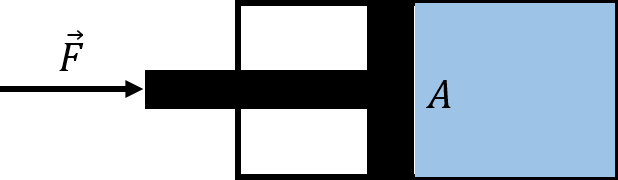
\includegraphics[width=0.4\linewidth]{files/piston-a5fa6b938507247d21d53e3029e31b09.png}
\caption[]{A force exerted on the piston will increase the pressure everywhere in the fluid.}
\label{fig:fluidmechanics:piston}
\end{figure}

If we wish to determine the absolute pressure in the water at some depth, $h$, in the ocean, we need to include the fact that the Earth's atmosphere exerts a net downwards force on the surface of the ocean in addition to the fact that the pressure changes with depth due to gravity. The pressure from the air in the Earth's atmosphere is called ``atmospheric pressure'', and depends on a variety of conditions, such as the weather. The average pressure from the atmosphere is $P_0=1.013\times 10^5 {\rm Pa}$. If the atmospheric pressure is $P_0$ at the surface of the ocean, then the pressure at some depth, $h$, is given by:
\begin{equation}
P(h) = P_0 + \rho g h
\end{equation}
where $\rho$ is the density of water. As a consequence, the pressure at any depth, $h$, in a fluid is the same everywhere at that depth in the fluid.

\begin{framed}
\textbf{Checkpoint}\\
\begin{figure}[!htbp]
\centering
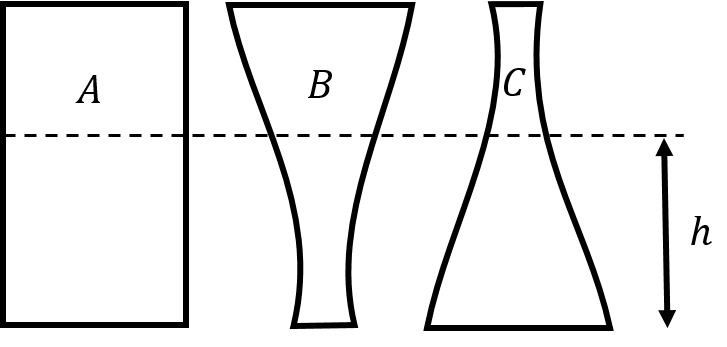
\includegraphics[width=0.4\linewidth]{files/glasses-f971074bb518c1c63523f0c7b808c680.png}
\caption[]{Three glasses with different shapes.}
\label{fig:fluidmechanics:glasses}
\end{figure}

You fill the three glasses in Figure~\ref{fig:fluidmechanics:glasses} such that the liquid reaches a height $h$ above the bottom of the glass. What can you say about the pressure of the liquid at the bottom of each glass?

\begin{enumerate}
\item It is highest for glass $A$.
\item It is highest for glass $B$.
\item It is highest for glass $C$.
\item It is the same for all glasses.
\item It is only the same for all glasses if we can neglect atmospheric pressure.
\end{enumerate}

\begin{framed}
\textbf{Answer}\\
\begin{enumerate}[resume]
\item
\end{enumerate}
\end{framed}
\end{framed}

\begin{framed}
\textbf{Example 14.2}\\
\begin{figure}[!htbp]
\centering
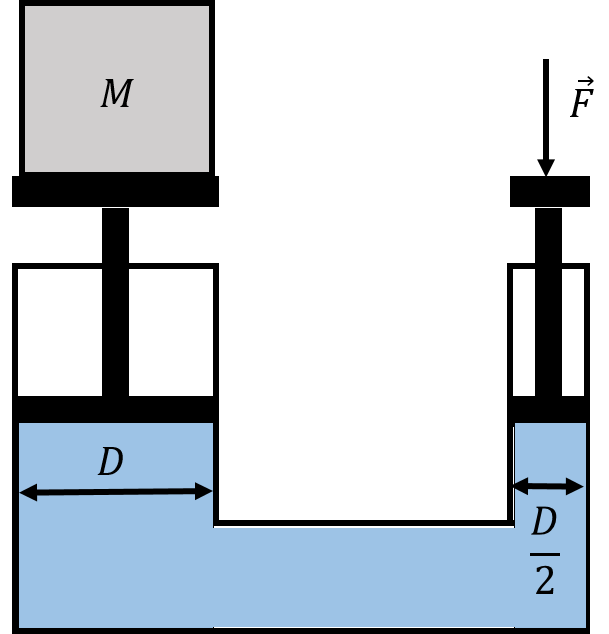
\includegraphics[width=0.4\linewidth]{files/lift-44b21302d3cbe001ed1715eb06d547c5.png}
\caption[]{A force exerted on the piston of a hydraulic lift in order to lift a mass $M$.}
\label{fig:fluidmechanics:lift}
\end{figure}

A hydraulic lift exploits Pascal's principle in order to use a small force to exert a large force. The hydraulic lift in Figure~\ref{fig:fluidmechanics:lift} shows a lift that is constructed by having a fluid between two vertical movable pistons. The pistons are cylindrical and the diameter of their cross-sections are $D$ and $D/2$. A mass, $M$, is placed on the piston with the larger diameter. What is the magnitude of the force, $\vec F$, that must be applied on the smaller piston in order to lift the mass, $M$?

\begin{framed}
\textbf{Solution}\\
If a force $\vec F$ is applied to the small piston, then the pressure in the fluid will increase by:
\begin{equation}
\Delta P = \frac{F}{A}=\frac{F}{\pi \frac{D^2}{4}}=\frac{4F}{\pi D^2}
\end{equation}
This will result in a net upwards force, $\vec F'$, on the large piston, with a magnitude:
\begin{equation}
F' = \Delta P A' = \Delta P \pi D^2 = \frac{4F}{\pi D^2} \pi D^2 = 4F
\end{equation}
Thus the force on the large piston will be four times that exerted on the small piston. One only needs to exert a force with a magnitude of $Mg/4$ in order to lift the mass, $M$.
\end{framed}
\end{framed}

\paragraph{Measuring pressure}

In this section, we describe how one can design instruments to measure pressure. The most straightforward device is a manometer, which is constructed using a U-shaped tube filled with a fluid of known density, $\rho$, as shown in Figure~\ref{fig:fluidmechanics:manometer}.

\begin{figure}[!htbp]
\centering
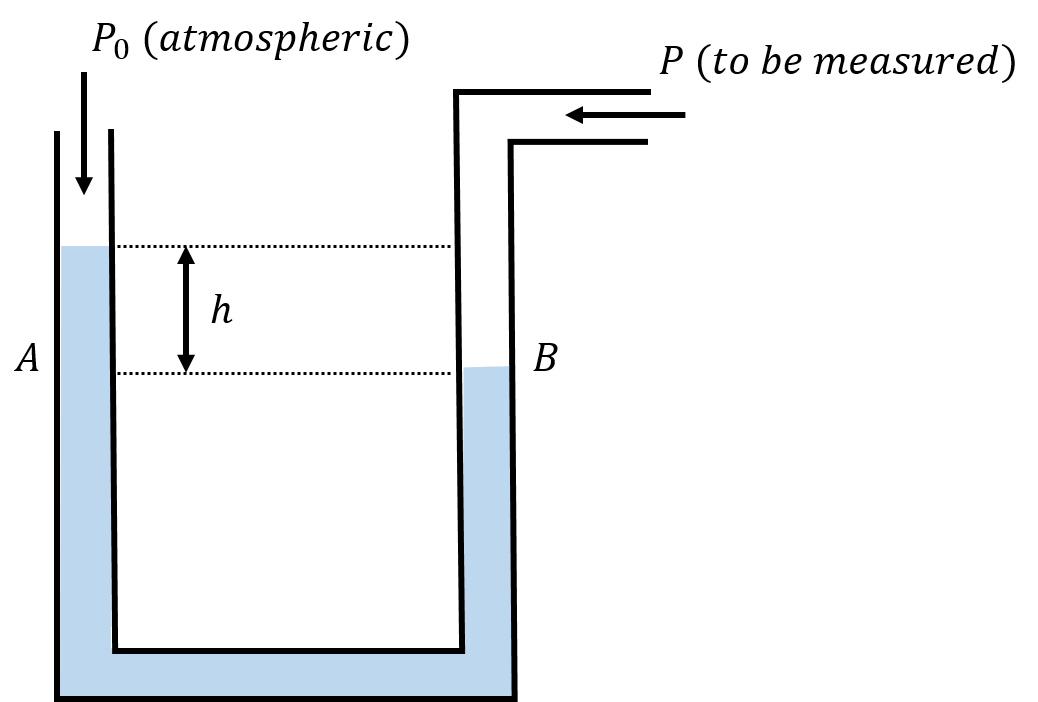
\includegraphics[width=0.65\linewidth]{files/manometer-2dfb021d7a68dc0d4b34f2cb901c2913.png}
\caption[]{A manometer can measure the difference between a pressure $P$ and atmospheric pressure, $P_0$. That difference is called ``gauge pressure''.}
\label{fig:fluidmechanics:manometer}
\end{figure}

A manometer can be used to measure a pressure $P$ relative to atmospheric pressure, $P_0$. One end of the tube is open to atmospheric pressure, and the other is connected to the fluid (e.g. a gas) for which we want to measure the pressure. If the pressure being measured is larger than atmospheric pressure, the fluid in the manometer will experience a greater downwards force on the side of the pressure to be measured than on the side open to atmospheric pressure, as shown in Figure~\ref{fig:fluidmechanics:manometer}. There will be a difference, $h$, in the level of the fluid on each side of the tube, which is directly proportional to the difference in pressure between the two sides of the tube.

Consider the point in the fluid at location $B$ in Figure~\ref{fig:fluidmechanics:manometer}, where the pressure is $P_B=P$, the pressure to be measured. The point in the fluid at location $A$, which is at the same height in the fluid, must have the same pressure as point $B$. We can write the pressure at point $A$, $P_A$, as the sum of the atmospheric pressure and the pressure from the column of water of height, $h$:
\begin{equation}
P_A=P_0+\rho g h
\end{equation}
Since this must also be equal to the pressure at point $B$, we can find the difference between the pressure we want to measure and atmospheric pressure:
\begin{equation}
P_A &= P_B \\
P_0+\rho g h &= P\\
\therefore P - P_0 &= \rho g h
\end{equation}
The difference between a pressure and the atmospheric pressure is called ``gauge pressure'', and is all that we can measure if we do not know the absolute value of the atmospheric pressure. Using a manometer, the gauge pressure is given by $\rho g h$, whereas the ``absolute pressure'', $P$, is given by adding the atmospheric pressure to the gauge pressure, $P = P_0 + \rho g h$. Most pressure measuring devices (``pressure gauges''), measure pressure relative to atmospheric pressure, using a similar mechanism.

The atmospheric pressure at a location on Earth varies based on the weather. A barometer is an instrument designed to measure the atmospheric pressure. A simple barometer can be built from a manometer, with one end closed, as illustrated in Figure~\ref{fig:fluidmechanics:barometer}.

\begin{figure}[!htbp]
\centering
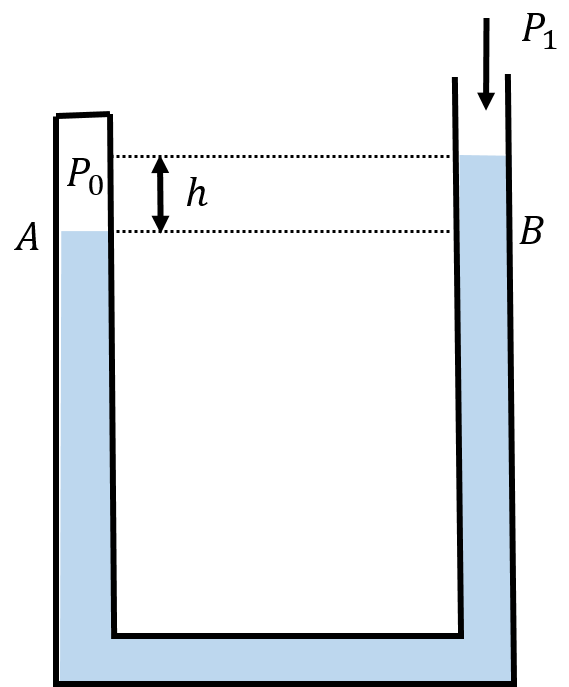
\includegraphics[width=0.3\linewidth]{files/barometer-85148bce6cdce1c2718b1ffccd8215e1.png}
\caption[]{A barometer constructed from a manometer to measure relative changes in atmospheric pressure.}
\label{fig:fluidmechanics:barometer}
\end{figure}

One end of the manometer is sealed on a day where the atmospheric pressure is, say, $P_0$, while the other end of the tube is left open. The height difference, $h$, between the fluid in either side of the tube is a measure of how different the current atmospheric pressure, $P_1$, is relative to the pressure, $P_0$, when the manometer was sealed. In Figure~\ref{fig:fluidmechanics:barometer}, the barometer is shown on a day where the atmospheric pressure is lower than on the day the manometer was sealed. The difference in pressure is given by:
\begin{equation}
P_1 = P_0 + \rho g h
\end{equation}
if we define $h$ to be positive when the side with the pressure $P_0$ is higher (so $h$ is negative in Figure~\ref{fig:fluidmechanics:barometer} and $P_1$ is less than $P_0$).

We can also measure the absolute atmospheric pressure if we evacuate the air out of the sealed end of the tube, so that $P_0=0$. When doing so, the difference in height between the fluid on either side of the manometer is a measure of the absolute atmospheric pressure.

\begin{framed}
\textbf{Example 14.3}\\
\begin{figure}[!htbp]
\centering
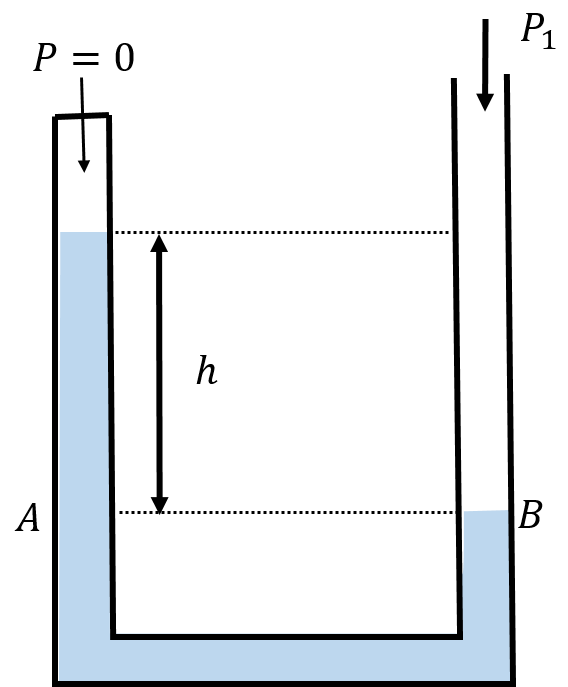
\includegraphics[width=0.3\linewidth]{files/barometer_abs-7a94d5b1571a753cbec3652d23ac0b05.png}
\caption[]{A barometer constructed from a manometer to measure absolute atmospheric pressure.}
\label{fig:fluidmechanics:barometer_abs}
\end{figure}

Using a manometer filled with water ($\rho=1\times 10^3 {\rm kg/m^3}$), you construct a barometer to measure the absolute atmospheric pressure by evacuating the air from one side of the manometer, as shown in Figure~\ref{fig:fluidmechanics:barometer_abs}. What is the difference in height, $h$, when the atmospheric pressure is ``nominal'' $P_1=1.013\times 10^5 {\rm Pa}$?

\begin{framed}
\textbf{Solution}\\
The pressure, $P_1$, on the open side of the manometer is given by:
\begin{equation}
P_B &= P_A\\
P_1&= P_0 + \rho g h = \rho g h
\end{equation}
if the sealed side of the manometer has a pressure, $P_0=0$, above the fluid. If $P_1=1.013\times 10^5 {\rm Pa}$, we can find the height, $h$:
\begin{equation}
h=\frac{P_1}{\rho g}=\frac{(1.013\times 10^5 {\rm Pa})}{(1000 {\rm kg/m^3})(9.8 {\rm m/s^2})}=10.3 {\rm m}
\end{equation}
\textbf{Discussion:} The difference in height is about $10 {\rm m}$ when the atmospheric pressure is nominal. This means that the manometer needs to be at least this tall to measure absolute atmospheric pressure, which is not practical to construct! If, instead, one uses a liquid with a higher density than that of water, then this height can be reduced substantially. Traditionally, barometers have been built using mercury, which has a density of ($\rho_{Hg}= 13.6\times 10^3 {\rm kg/m^3}$), so that the height difference at nominal atmospheric pressure is $760 {\rm mm}$. This is a much easier instrument to build (apart from the safety concerns of using mercury). For this reason, an often-used unit of pressure is ``mm of mercury'', which corresponds to the height difference in a manometer that is built using mercury.
\end{framed}
\end{framed}

\begin{framed}
\textbf{Checkpoint}\\
\begin{figure}[!htbp]
\centering
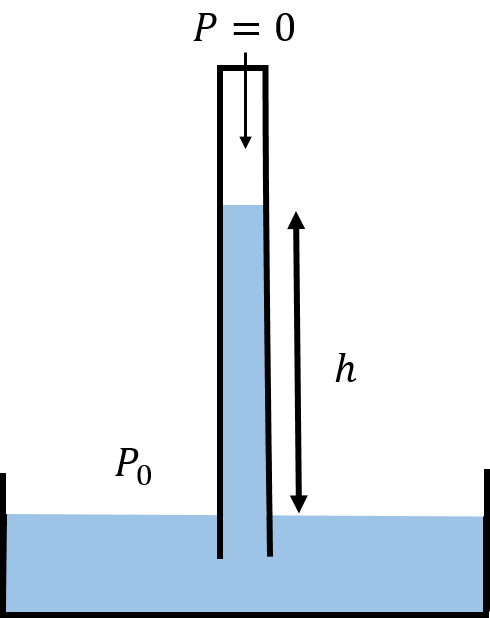
\includegraphics[width=0.3\linewidth]{files/barometer2-ce29b35f970087027dde88afe61f9b72.png}
\caption[]{A Torricelli barometer.}
\label{fig:fluidmechanics:barometer2}
\end{figure}

You build a Torricelli barometer, as illustrated in Figure~\ref{fig:fluidmechanics:barometer2}, to measure the absolute atmospheric pressure. The sealed vertical tube has a space at the top that is evacuated (a pressure of zero), so that atmospheric pressure on the container of liquid forces the liquid up the tube to a height, $h$, which is proportional to atmospheric pressure. If you use olive oil as the liquid, what can you say about the height, $h$, for nominal atmospheric pressure?

\begin{enumerate}
\item It is greater than $10.3 {\rm m}$.
\item It is equal to $10.3 {\rm m}$.
\item It is less than $10.3 {\rm m}$.
\item Not enough information to tell.
\end{enumerate}

\begin{framed}
\textbf{Answer}\\
\begin{enumerate}
\item
\end{enumerate}
\end{framed}
\end{framed}

\subsubsection{Buoyancy}

In this section, we examine how the pressure gradient in a fluid leads to a force of buoyancy on an object that is immersed in the fluid.

\begin{figure}[!htbp]
\centering
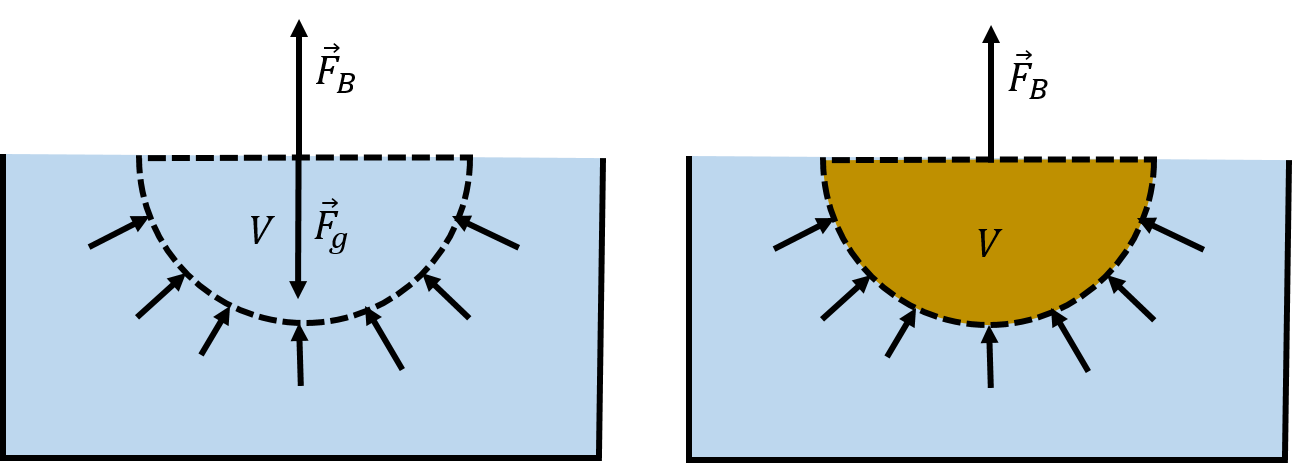
\includegraphics[width=0.7\linewidth]{files/buoyant-ea529a7a112b2f4a49686e7f9a49e604.png}
\caption[]{(Left:) The weight of a fluid element, $\vec F_g$, is supported by the net upwards force from the pressure, $\vec F_B$, of the fluid below it. (Right:) If the fluid element is removed and replaced with an object, there will still be the same net upwards force, $\vec F_B$, from the pressure of the fluid, which is now exerted on the object.}
\label{fig:fluidmechanics:buoyant}
\end{figure}

In the left panel of Figure~\ref{fig:fluidmechanics:buoyant}, we show a hemi-spherical element of fluid with a volume $V$. The weight of the element of fluid, $\vec F_g$, is supported by the net upwards force, $\vec F_B$, exerted by the pressure of the fluid surrounding the fluid element. The mass, $M$, of the element of fluid is given by:
\begin{equation}
M = \rho V
\end{equation}
where $\rho$ is the density of the fluid. The net force from the pressure, $F_B$, must thus have the same magnitude as the weight:
\begin{equation}
F_B = Mg = \rho V g
\end{equation}
Now, suppose that the fluid element is ``displaced'' and replaced by the hull of a boat, as shown in the right panel of Figure~\ref{fig:fluidmechanics:buoyant}. The net upwards force from the pressure of the fluid must remain the same, $F_B$, but that force is now exerted on the hull of the boat. We call that force the force of ``buoyancy'', which is the reason that a boat can float and the reason that you feel lighter when walking in a swimming pool than on land.

Thus, if an object displaces a volume, $V$, of a fluid with density $\rho$, when immersed in the fluid, that object will experience an upwards force of buoyancy, $\vec F_B$, with magnitude:
\begin{equation}
\boxed{F_B = \rho V g}
\end{equation}
This ``principle'' was originally discovered by Archimedes, who stated that the force of buoyancy is equal to the weight of the displaced fluid. Note that we drew the fluid element at the surface of the fluid, but this is not required, and a force of buoyancy will be present if the object is completely immersed in the liquid. If you refer back to Figure~\ref{fig:fluidmechanics:pressure_gravity}, you will recall that the net upwards force on an element of fluid must be equal to its weight, even if the fluid element is completely immersed.

\begin{framed}
\textbf{Checkpoint}\\
Does the force of buoyancy on a fully submerged object increase with the depth at which the object is submerged (ignoring any change from the varying value of $\vec g$)?

\begin{enumerate}
\item Yes, because the force of buoyancy comes from the pressure in the fluid, which increases with depth.
\item No, because the force of buoyancy comes from the difference in pressure above and below the object, which does not increase with depth.
\end{enumerate}

\begin{framed}
\textbf{Answer}\\
\begin{enumerate}[resume]
\item
\end{enumerate}
\end{framed}
\end{framed}

\begin{framed}
\textbf{Checkpoint}\\
You observe that if you pour olive oil slowly into your glass of water, the oil floats above the water. What can you conclude?

\begin{enumerate}
\item The mass of a given volume of oil is less than the mass of the same volume of water.
\item The mass of a given volume of oil is more than the mass of the same volume of water.
\end{enumerate}

\begin{framed}
\textbf{Answer}\\
\begin{enumerate}
\item
\end{enumerate}
\end{framed}
\end{framed}

\begin{framed}
\textbf{Example 14.4}\\
You measure the weight of an object by suspending it with a spring scale. When you measure the weight of the object in air, you find that it has a weight $W_{a}$. When you measure the weight of the object when it is completely submerged in water, you find that it has a weight $W_w$. What is the density of the object?

\begin{framed}
\textbf{Solution}\\
Given the weight of the object in air, we can easily determine its mass:
\begin{equation}
M = \frac{W_a}{g}
\end{equation}
However, since we do not know its volume, $V$, we cannot directly determine its density. When the object is submerged in water, the measured weight will be the actual weight of the object (as measured in air) minus the magnitude of the force of buoyancy exerted by the water:
\begin{equation}
W_w &= W_a - \rho_w g V\\
\therefore V &= \frac{W_a -W_w}{\rho_w g}
\end{equation}
where $\rho_w$ is the density of water. Given the volume, we can now determine the object's density, $\rho$:
\begin{equation}
\rho = \frac{M}{V}=\frac{W_a\rho_w g}{g (W_a -W_w)}=\rho_w\frac{W_a}{W_a -W_w}
\end{equation}
\textbf{Discussion:} By using Archimedes' Principle, we were able to determine the volume, and thus the density of the object, by comparing measurements of its weight in air and in water. This is similar to the method that Archimedes came up with to determine if a crown owned by a general was made of real gold or if some of the gold had been replaced with an equal weight of silver. Archimedes supposedly went to the baths to ponder how to determine if the crown was made of gold and had his Eureka moment when we he noticed the water level in the bath went up as he went into the bath. He realized that denser gold would displace less water than silver for an equal weight.
\end{framed}
\end{framed}

\begin{framed}
\textbf{Olivia's Thoughts}\\
Whether or not an object will float depends on its density. Let's consider an object that is placed in water. The only forces acting on the object are its weight and the force of buoyancy. We want to know when the net force will be zero. I'm going to write out Newton's Second Law for the object, but writing the mass of the object in terms of its density and volume.
\begin{equation}
F_g&=F_B\\
m_Og&=F_B\\
\rho_OV_Og&=\rho_WV_Wg
\end{equation}
where $O$ refers to the object and $W$ refers to the water. Cancelling out the $g$'s, we can write this as:
\begin{equation}
\frac{\rho_O}{\rho_W}=\frac{V_W}{V_0}
\end{equation}
Consider a solid cube that has the same density as water. In this case, $\rho_0/\rho_W=1$, and so $V_W/V_0=1$. This means that, in order for the cube to float, a volume of water that is equal to the volume of the cube must be displaced. So, the entire cube must be submerged. If you placed this cube 5 \{{\textbackslash}rm m\} deep in the water, it would stay at this depth.

Now consider a cube whose density is half that of water. We find that $\rho_0/\rho_W=0.5$, so we must have $V_W/V_0=0.5$. In order for the cube to float, only half of it needs to be submerged. If you placed the cube $5 {\rm m}$ deep in the water, it would rise to the surface and stop when half of it was above water (after bobbing for a bit).

Finally, what about a cube whose density is 1.5 times the density of water? In this case, one and a half cubes worth of water would have to be displaced in order for the cube to float. Even when the entire cube is submerged, not enough volume has been displaced in order for it to float, so the cube will sink.

Objects like pool noodles or life jackets allow us to float because they have low densities. They have very little mass (they don't add much to the weight) in a relatively large volume (they can displace water to add to the buoyant force). An object with a density less than water will float with some fraction of the object being submerged.
\end{framed}

\subsubsection{Hydrodynamics}

In the previous sections we developed ``hydrostatic'' models for fluids when those fluids are at rest (in some inertial reference frame). In this section, we develop ``hydrodynamic'' models to discuss what happens when fluids flow. We will restrict our models to fluids that flow in a ``laminar'' fashion, rather than a ``turbulent'' fashion.

Laminar flow is the flow of a fluid when each particle in the fluid follows a path that can be represented by a line (a ``streamline''). Turbulent flow is the flow of a fluid where particles can follow rather complex paths, usually involving ``Eddy currents'' (little whirlpools). The two types of flow are illustrated in Figure~\ref{fig:fluidmechanics:turbulent}.

\begin{figure}[!htbp]
\centering
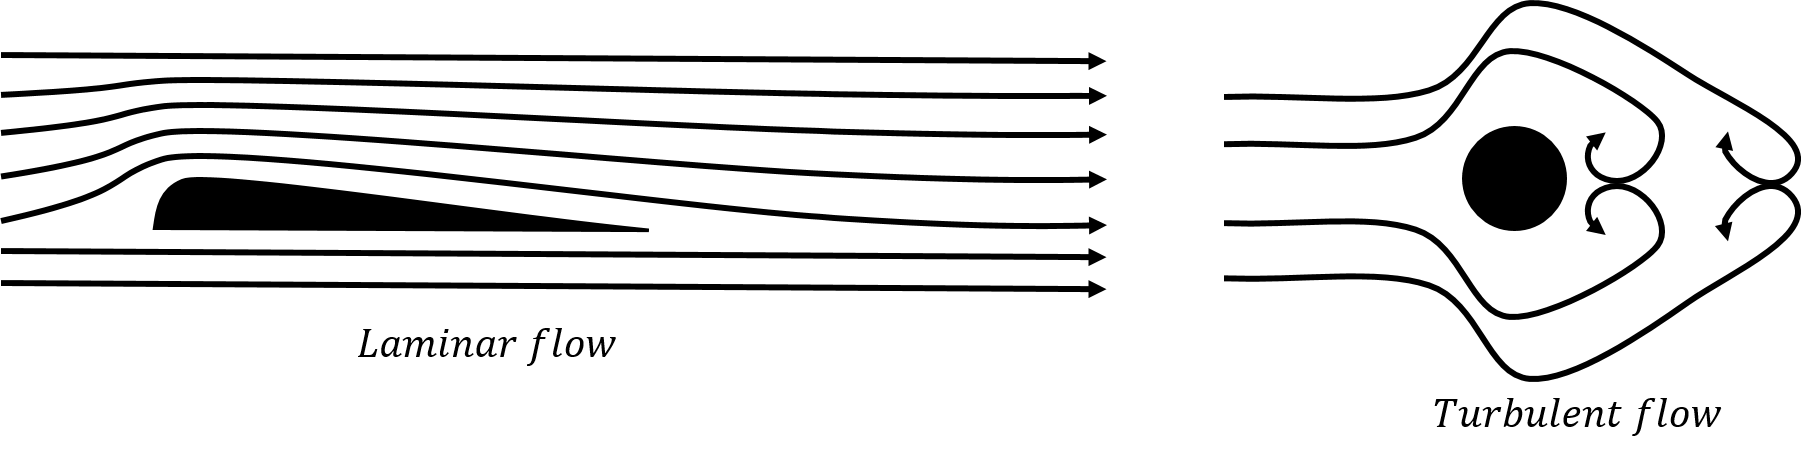
\includegraphics[width=0.7\linewidth]{files/turbulent-3667d33728ed1bb7e6ff66cd9ff97f34.png}
\caption[]{Laminar (left) and turbulent (right) flow of a fluid around an object.}
\label{fig:fluidmechanics:turbulent}
\end{figure}

\paragraph{Continuity of flow}\label{sec:fluidmechanics:continuity}

Consider the laminar flow of a fluid through a pipe whose cross-sectional area narrows from $A_1$ to $A_2$ in the direction of flow, as illustrated in Figure~\ref{fig:fluidmechanics:continuous}.

\begin{figure}[!htbp]
\centering
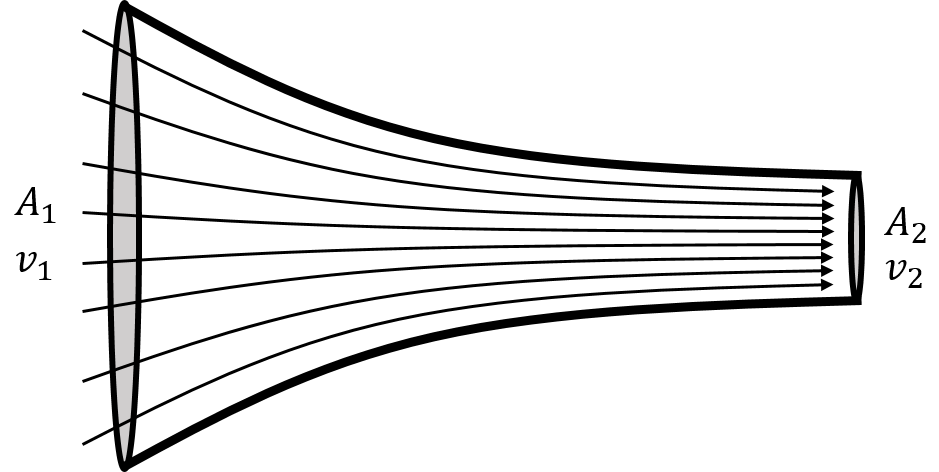
\includegraphics[width=0.6\linewidth]{files/continuous-9fe71e3af537f52ce783298d23745ef9.png}
\caption[]{Laminar flow of a fluid in a narrowing pipe.}
\label{fig:fluidmechanics:continuous}
\end{figure}

The particles that make up the fluid have a speed $v_1$ at the wide end of the pipe and speed $v_2$ at the narrow end. The \textbf{equation of continuity} is based on the premise that the fluid that enters the pipe must exit the pipe, as there is nowhere else for the fluid to go. That is, if during a period of time, $\Delta t$, a mass, $\Delta m$, of fluid enters the wide end of the pipe, then during that same period of time, the same mass of fluid must exit the narrow end of the pipe.

During a period of time, $\Delta t$, the fluid at the wide end of the pipe will travel a distance $l_1=v_1\Delta t$. Thus, a volume of fluid, $\Delta V_1$, will enter the wide end of the pipe:
\begin{equation}
\Delta V_1 = A_1 l_1 = A_1 v_1 \Delta t
\end{equation}
Similarly, during that period of time, a volume $\Delta V_2$ will exit the narrow end of the pipe:
\begin{equation}
\Delta V_2 = A_2 l_2 = A_2 v_2 \Delta t
\end{equation}
If the fluid is compressible, its density can change. Let $\rho_1$ be the density of the fluid at the wide end of the pipe and $\rho_2$ be the density of the fluid at the narrow end. The mass of fluid, $\Delta m$, entering the wide end of the pipe is given by:
\begin{equation}
\Delta m = \rho_1 \Delta V_1= \rho_1 A_1 v_1 \Delta t
\end{equation}
The mass of fluid exiting the narrow end of the pipe is given by:
\begin{equation}
\Delta m = \rho_2 \Delta V_2= \rho_2 A_2 v_2 \Delta t
\end{equation}
The mass of fluid entering the wide end of the pipe must equal the mass exiting the narrow end of the pipe:
\begin{equation}
\rho_1 A_1 v_1 \Delta t &= \rho_2 A_2 v_2 \Delta t
\end{equation}
Leading to the equation of continuity:
\begin{equation}
\boxed{\rho_1 A_1 v_1 = \rho_2 A_2 v_2}
\end{equation}
The quantity $\rho A v$ has dimensions of mass per time, and corresponds to the mass of fluid passing through a cross section $A$ per unit time.

If the fluid is incompressible, as are most liquids, then the density is the same on both sides of the pipe, and the equation simplifies to:
\begin{equation}
\boxed{A_1 v_1 = A_2 v_2}\quad\text{(Incompressible fluid)}
\end{equation}
For a liquid, we can define the ``volumetric flow'', $Q$, as:
\begin{equation}
Q=Av
\end{equation}
where $A$ is the cross-sectional area of the surface through which a fluid with speed, $v$, flows\footnote{If the velocity of the fluid is not perpendicular to the surface, then $v$ is the component of the velocity perpendicular to the surface.}. $Q$ has the dimension of volume per time, and corresponds to the volume of fluid passing through the cross section $A$ per unit time. For an incompressible fluid, the equation of continuity is thus equivalent to stating that the volumetric flow, $Q$, of the fluid is a constant.

\begin{framed}
\textbf{Checkpoint}\\
\begin{figure}[!htbp]
\centering
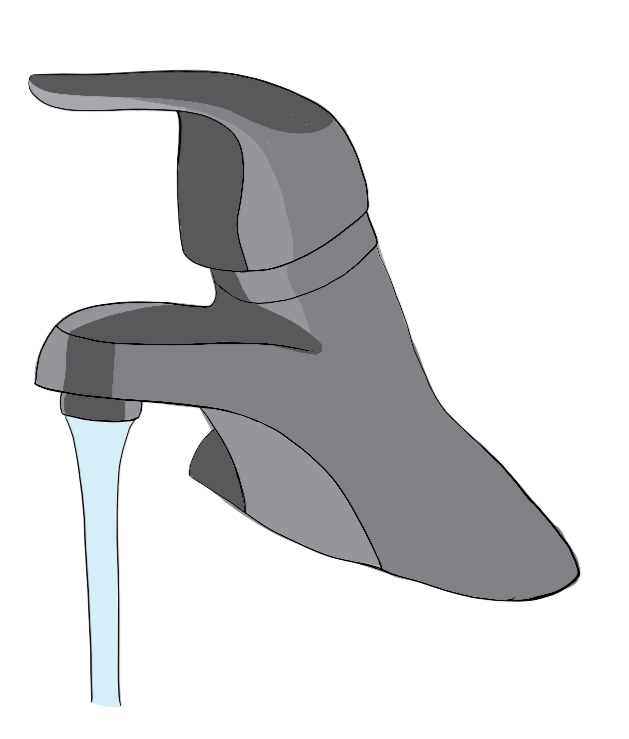
\includegraphics[width=0.2\linewidth]{files/necking-9c723b4df639509caf658d10ea8c0700.png}
\caption[]{Water flowing out of a faucet.}
\label{fig:fluidmechanics:necking}
\end{figure}

When water flows out of your faucet, you observe that the stream of water gets narrower as the water moves down, as shown in Figure~\ref{fig:fluidmechanics:necking}. Why is this?

\begin{enumerate}
\item The atmospheric pressure increases as the waters moves downwards, so the stream of water is more and more compressed.
\item As the water accelerates due to gravity, the cross-sectional area of the flowing water must reduce in order to preserve a constant flow rate.
\end{enumerate}

\begin{framed}
\textbf{Answer}\\
\begin{enumerate}[resume]
\item
\end{enumerate}
\end{framed}
\end{framed}

\begin{framed}
\textbf{Example 14.5}\\
Your garden hose has a diameter of $D=2 {\rm cm}$. How fast must water flow out of the hose if you are to fill a $5 {\rm l}$ bucket in one minute?

\begin{framed}
\textbf{Solution}\\
We need the volume flow rate from the hose to be $Q=5 {\rm l/min}$. We can convert this to SI units:
\begin{equation}
Q=(5 {\rm l/min})\left(\frac{1}{1000}{\rm m^3/l}\right) \left(\frac{1}{60}{\rm min/s}\right)=\frac{5}{6\times 10^4}{\rm m^3/s}=8.3\times 10^{-5} {\rm m^3/s}
\end{equation}
Since we know the area of the hose, we can determine the speed of the water to achieve the given flow rate:
\begin{equation}
Q &= Av=\pi \left(\frac{D}{2}\right)^2v \\
\therefore v&=\frac{Q}{\pi \left(\frac{D}{2}\right)^2}=\frac{(8.3\times 10^{-5} {\rm m^3/s})}{\pi(0.01 {\rm m})^2}=0.265 {\rm m/s}
\end{equation}
\end{framed}
\end{framed}

\paragraph{Bernoulli's Principle}

In this section, we examine how the pressure and speed of a fluid change as the fluid flows. We will restrict ourselves to discussing the \textbf{laminar} flow of an \textbf{incompressible} fluid with no friction. Bernoulli was the first to quantitatively describe the flow of incompressible fluids, and we will show in this section how to derive ``Bernoulli's Principle''.

Consider the laminar flow of an incompressible fluid through a pipe that changes height, from $y_1$ to $y_2$, as well as cross-sectional area, from $A_1$ to $A_2$, as shown in Figure~\ref{fig:fluidmechanics:bernoulli}. The figure shows an element of fluid, in blue, as it moves through the pipe. The top panel corresponds to the location of the fluid element at time $t=0$, whereas the bottom panel shows the location of the element of fluid at time $t=\Delta t$.

\begin{figure}[!htbp]
\centering
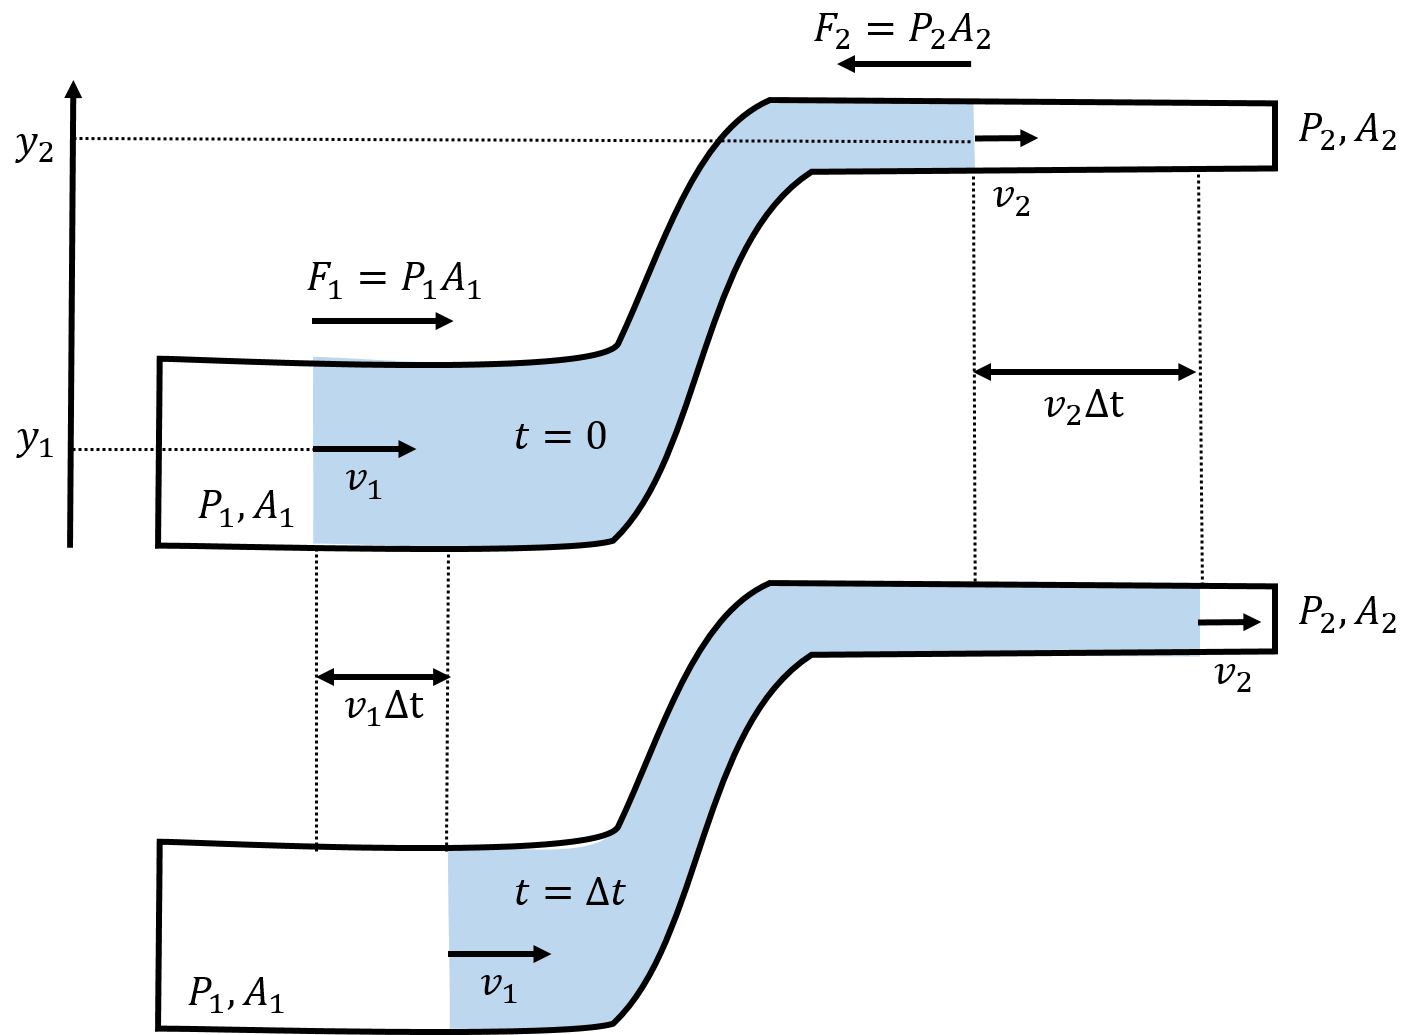
\includegraphics[width=0.75\linewidth]{files/bernoulli-8c7fea6b2fce6353b9fa7800c80cbf33.png}
\caption[]{Laminar flow of an incompressible fluid through a pipe that changes cross-sectional area and height in the direction of flow. An element of fluid, in blue, is shown at time $t=0$ (top panel), and then, at a later time, $t=\Delta t$ (bottom panel).}
\label{fig:fluidmechanics:bernoulli}
\end{figure}

To model how the fluid moves through this pipe, we can use energy and the Work-Energy Theorem. We start by considering the amount of work done on the element of fluid as it moves from the position in the top panel to the position in the bottom panel.

The fluid that is to the left of the element of fluid exerts a pressure, $P_1$, on the fluid element that leads to a net force, $\vec F_1$, towards the right. Similarly, the fluid to the right of the element of fluid exerts a net force $\vec F_2$ in the opposite direction, due to the pressure $P_2$ on that side of the fluid element.

In a period of time, $\Delta t$, the left part of the fluid element will move a distance $l_1 = v_1 \Delta t$, while the right part of the fluid element will move a distance $l_2=v_2\Delta t$. We can calculate the work done by each force, defining positive work to be in the direction of motion:
\begin{equation}
W_1 &=  F_1l_1 = (P_1A_1)(v_1 \Delta t)\\
W_2 &= -F_2l_2 = -(P_2A_2)(v_2 \Delta t)
\end{equation}
Gravity will also do (negative) work on the fluid as it changes height. In a period of time, $\Delta t$, a mass of fluid, $\Delta m$, will move from position $y=y_1$ to position $y=y_2$. The mass of fluid that changes height is given by the part of the fluid that moves a distance, $l_1$, on the right side of the pipe:
\begin{equation}
\Delta m = V_1 \rho = A_1 l_1 \rho = A_1 v_1 \Delta t \rho
\end{equation}
Because of the equation of continuity, this is also equal to the mass of fluid that moves a distance, $l_2$, on the left side of the pipe:
\begin{equation}
\Delta m = V_2 \rho = A_2 l_2 \rho = A_2 v_2 \Delta t \rho
\end{equation}
since $A_1v_1 = A_2 v_2$.

The force of gravity will thus do negative work on that mass element:
\begin{equation}
W_g = -\Delta m g (y_2-y_1) = -(A_1 v_1 \Delta t \rho) g (y_2-y_1)
\end{equation}
The net work done on the element of fluid over the time $\Delta t$ is thus:
\begin{equation}
W^{net} &= W_1+W_2+W_g = P_1A_1v_1 \Delta t - P_2A_2v_2 \Delta t -A_1 v_1 \Delta t \rho g (y_2-y_1)
\end{equation}
Note that, because of the equation of continuity, $A_1v_1 = A_2 v_2$, we can factor out a $A_1v_1$ from each term:
\begin{equation}
W^{net} &=A_1v_1 \Delta t \Bigl(P_1- P_2 - \rho g (y_2-y_1)\Bigr)
\end{equation}
The net work done on the fluid must equal the change in kinetic energy, $\Delta K$, of the mass element, $\Delta m$, from one end of the pipe to the other:
\begin{equation}
\Delta K &= \frac{1}{2}\Delta m v_2^2 - \frac{1}{2}\Delta m v_1^2\\
&=\frac{1}{2}( A_1 v_1 \Delta t \rho) (v_2^2 - v_1^2)
\end{equation}
Using the Work-Energy Theorem, we have:
\begin{equation}
W^{net} &=\Delta K\\
A_1v_1 \Delta t \Bigl(P_1- P_2 - \rho g (y_2-y_1)\Bigr) &= \frac{1}{2}( A_1 v_1 \Delta t \rho) (v_2^2 - v_1^2)\\
P_1 - P_2 - \rho g (y_2-y_1)&= \frac{1}{2}\rho v_2^2 - \frac{1}{2}\rho v_1^2
\end{equation}
We can re-arrange this so that all the quantities for each side of the pipe are on the same side of the equation:
\begin{equation}
P_1 +\frac{1}{2}\rho v_1^2+ \rho g y_1= P_2 + \frac{1}{2}\rho v_2^2 + \rho g y_2
\end{equation}
Since the locations 1 and 2 that we chose are arbitrary, we can state that, for laminar incompressible flow, the following quantity evaluated at any position is a constant:
\begin{equation}
\boxed{P +\frac{1}{2}\rho v^2+ \rho g y=\text{constant}}
\end{equation}
This statement is what we call Bernoulli's Equation, and is equivalent to conservation of energy for the fluid. If the fluid is not flowing ($v_1=v_2=0$), then this is equivalent to the statement of hydrostatic equilibrium that we derived in (\ref{eq:fluidmechanics:pgrav}):
\begin{equation}
P_1 + \rho g y_1= P_2 + \rho g y_2\\
\therefore P_2 - P_1 = - \rho g (y_2 - y_1)
\end{equation}
If the flow of the fluid is at constant height ($y_2=y_1$), then Bernoulli's equation can be written as:
\begin{equation}
P_1 +\frac{1}{2}\rho v_1^2 = P_2 + \frac{1}{2}\rho v_2^2
\end{equation}
If a fluid is flowing at constant height such that $v_2 > v_1$ (as in Figure~\ref{fig:fluidmechanics:continuous}), then $P_2<P_1$; that is, the \textbf{pressure in the fluid is lower if the fluid is flowing faster}. Note that $P$ is the pressure inside the fluid and is not related to the force that would be exerted by the fluid if it were to collide with an object. It makes sense that the fluid has a lower pressure where it is moving faster, because the net force exerted on the fluid is related to the difference in pressure on either side of the fluid. The fluid will accelerate in the direction where pressure decreases, thus it will be moving faster when it is in a region of low pressure.

Bernoulli's principle can be used to describe many phenomena. For example, an airplane wing (technically, an ``airfoil'') creates lift because the pressure of the air above the wing is lower than the pressure of the air below the wing. This is illustrated in Figure~\ref{fig:fluidmechanics:airfoil}, which shows that the laminar flow of the air creates a low pressure area above the wing. As the stream lines of air encounter the wing, those that are above the wing get compressed together, which leads to a faster speed of the air above the wing (equation of continuity). The resulting difference in air pressure above and below the wing results in a net upwards force on the wing.

\begin{figure}[!htbp]
\centering
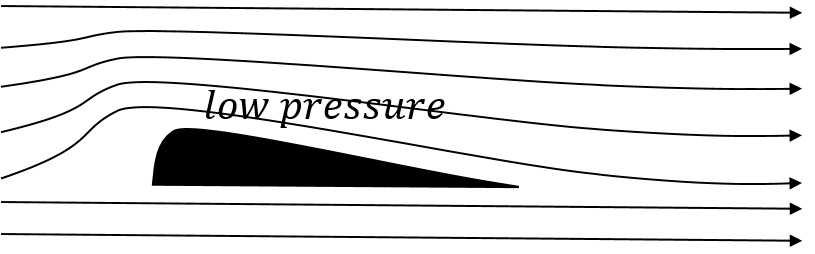
\includegraphics[width=0.5\linewidth]{files/airfoil-d539a074e9b004c12ca6bf5772a0b8bd.png}
\caption[]{Laminar flow of air around a airfoil. The curvature of the asymmetric airfoil forces the streamlines above the airfoil together, increasing the speed of the air due to the continuity equation, and resulting in a low pressure area.}
\label{fig:fluidmechanics:airfoil}
\end{figure}

Bernoulli's principle also describes why the roof can be lifted off of a house in high winds (Figure~\ref{fig:fluidmechanics:roof}, left panel). It is not the force of the wind against the roof that blows the roof off of a house; it is the difference in air pressure in the house (normal) and the pressure above the roof (low, due to the flowing wind), that results in a net upwards force on the roof. Bernoulli's principle is also used to construct atomizers which allow liquid in a bottle to be sprayed (Figure~\ref{fig:fluidmechanics:roof}, right panel). For example, perfume bottles often have a bulb connected to a tube/spout. When you squeeze the bulb, it causes the air in the tube to flow quickly, creating a low pressure in the vertical segment of the spout. The liquid is forced up by the pressure in the bottle; once the liquid arrives in the fast flowing air, it is sprayed out along with the air.

\begin{figure}[!htbp]
\centering
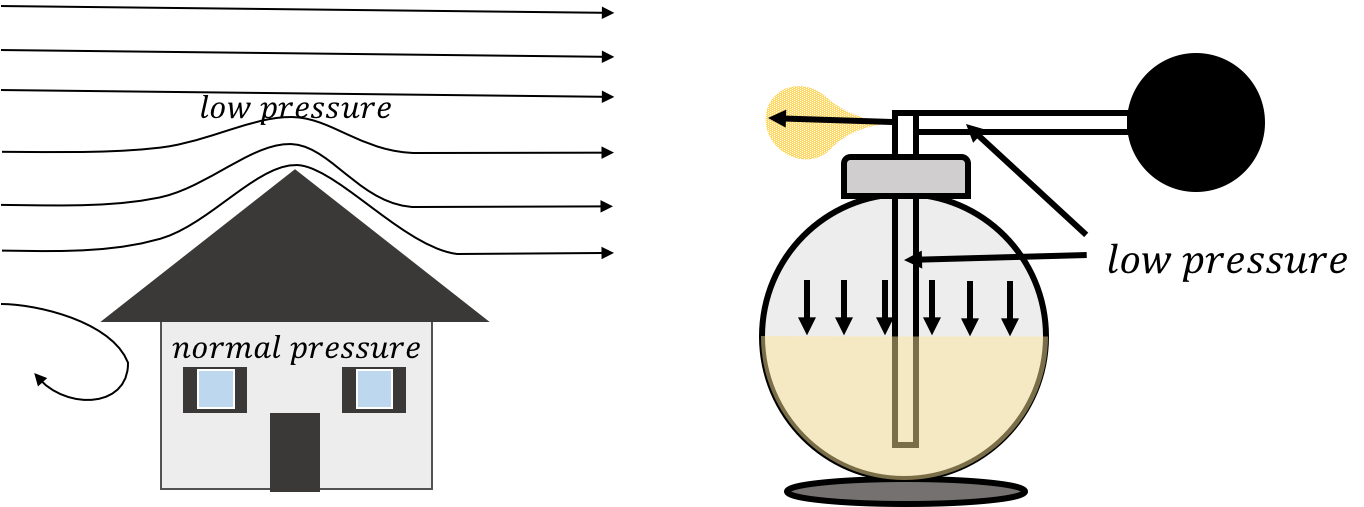
\includegraphics[width=0.8\linewidth]{files/roof-3ea62f3344fa6240b8d895f5aef03f78.png}
\caption[]{(Left:) the wind flowing above a roof creates a low pressure zone above the roof. (Right:) air flowing above a vertical spout in the atomizer creates a low pressure zone; the air pressure in the bottle forces the liquid up the spout.}
\label{fig:fluidmechanics:roof}
\end{figure}

\begin{framed}
\textbf{Checkpoint}\\
When a high speed train is travelling at constant speed, is there a net force on the windows from air pressure?

\begin{enumerate}
\item No, since the windows are stationary relative to the train, there is no net force on them from air pressure.
\item Yes, there is a net outwards force on the windows from air pressure.
\item Yes, there is a net inwards force on the windows from air pressure.
\end{enumerate}

\begin{framed}
\textbf{Answer}\\
\begin{enumerate}[resume]
\item
\end{enumerate}
\end{framed}
\end{framed}

The following examples illustrate how to apply Bernoulli's principle.

\begin{framed}
\textbf{Example 14.6}\\
\begin{figure}[!htbp]
\centering
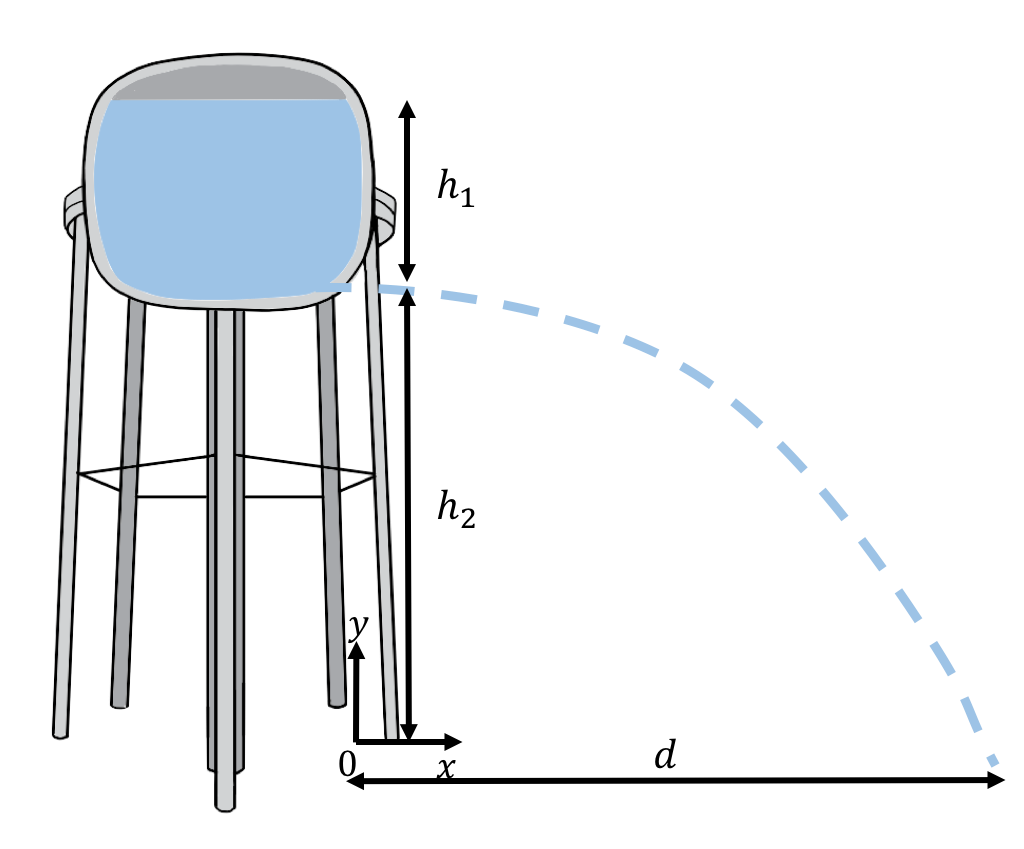
\includegraphics[width=0.4\linewidth]{files/watertower-bf14b826b3120c9b1f60adb113144920.png}
\caption[]{Water leaking out of a horizontal hole in a water tank.}
\label{fig:fluidmechanics:watertower}
\end{figure}

A water tower is constructed so that the bottom of the water tank is a height $h_2$ above the ground, as illustrated in Figure~\ref{fig:fluidmechanics:watertower}. The water in the tank is at a height $h_1$ from the bottom of the tank. A leak from a hole is found at the base of the tank (the water flows horizontally out of the hole). What is the horizontal distance, $d$, from the bottom of the tower to where the water from the leak hits the ground? Assume that the water level in the tank is constant and that atmospheric pressure does not change appreciably over the height of the tower.

\begin{framed}
\textbf{Solution}\\
The pressure in the water tank leads to the water exiting the bottom of the tank with a horizontal velocity of magnitude, $v$. That water then undergoes projectile motion on its way to the ground. We can first determine the speed of the water exiting the tank and then use the kinematics for projectile motion to model the distance, $d$.

We model the flow of the water using a two-dimensional coordinate system with a horizontal $x$ axis (positive to the right), and a vertical $y$ axis (positive upwards). We place the origin at the bottom of the water tower, on the ground, below the hole, as shown in Figure~\ref{fig:fluidmechanics:watertower}.

At the top of tank, at a height $y = h_1+h_2$, the water has a speed of zero and is at atmospheric pressure, $P_0$. At the exit of the hole at the bottom of the tank, at a height $y = h_2$, the water has a speed $v_2$ and is also at atmospheric pressure. Using Bernoulli's equation at the top (1) and bottom (2) of the tank, we have:
\begin{equation}
P_1 +\frac{1}{2}\rho v_1^2+ \rho g y_1&= P_2 + \frac{1}{2}\rho v_2^2 + \rho g y_2\\
P_0 + (0) + \rho g (h_1+h_2) &= P_0 +  \frac{1}{2}\rho v^2 + \rho g h_2\\
\therefore v_2 &= \sqrt{2gh_1}
\end{equation}
which is exactly the speed that any object falling a distance $h_1$ would have.

Using kinematics, we can find the time that it would take the water to fall a distance $h_2$ (where the water's velocity is horizontal as it exits the tank):
\begin{equation}
h_2 &= \frac{1}{2}gt^2\\
\therefore t &= \sqrt{\frac{2h_2}{g}}
\end{equation}
The distance $d$ covered by the water is thus given by:
\begin{equation}
d &= v_2t = \sqrt{2gh_1}\sqrt{\frac{2h_2}{g}} = \sqrt{4h_1h_2}
\end{equation}
\textbf{Discussion:} We find that the water coming out of the bottom of the tank, when there is a height, $h_1$, of water above it providing pressure, will have the same speed as that of a particle which has fallen a distance, $h_1$. This is because there is no net pressure difference between the top of the water tank and where the water has exited the hole, so gravity is the only force doing work on the water. Gravity will do work at the same rate on particles of water as on any other particle, so the speed of the water particles at the bottom of the tank is the same as if they had fallen a distance, $h_1$. Again, once the water particles are falling through the air, gravity is the only net force exerted on those particles, so they undergo projectile motion, just as any other particle would.
\end{framed}
\end{framed}

\begin{framed}
\textbf{Example 14.7}\\
You measure that water comes out of your kitchen faucet at a rate of $6 {\rm l/min}$. The faucet has a diameter of $2 {\rm cm}$. At what rate will water flow out of your basement faucet, which has a diameter of $1 {\rm cm}$ and is located a height, $h=3 {\rm m}$, below your kitchen faucet? Assume that atmospheric pressure, $P_0$, does not change appreciably between your kitchen and basement.

\begin{framed}
\textbf{Solution}\\
The water flows out of the kitchen faucet at a speed, $v_1$, where the pressure is atmospheric. If the area of the kitchen faucet is $A_1$ we can determine the speed, $v_1$, from the given flow rate, $Q_1=6 {\rm l/min}=1\times 10^{ -4} {\rm m^3/s}$:
\begin{equation}
Q_1 &= A_1 v_1\\
v_1 &= \frac{Q_1}{A_1}=\frac{(1\times 10^{-4} {\rm m^3/s})}{\pi (0.01 {\rm cm})^2}=0.318 {\rm m/s}
\end{equation}
The water will flow out of the basement faucet with a speed, $v_2$, where the pressure is also atmospheric, $P_0$. We can use Bernoulli's equation to relate the flow out of the basement faucet (2) to that at the kitchen faucet (1). We choose the $y$ axis of a vertical coordinate system such that the basement is located at $y_2=0$ and the kitchen faucet is located at $y_1=3 {\rm m}$:
\begin{equation}
P_1 +\frac{1}{2}\rho v_1^2+ \rho g y_1&= P_2 + \frac{1}{2}\rho v_2^2 + \rho g y_2\\
P_0+\frac{1}{2}\rho v_1^2+ \rho g y_1&= P_0 + \frac{1}{2}\rho v_2^2 \\
\frac{1}{2} v_1^2+  gy_1&=  \frac{1}{2} v_2^2 \\
\therefore v_2 &= \sqrt{v_1^2 + 2gy_1}\\
&=\sqrt{(0.318 {\rm m/s})^2+2(9.8 {\rm m/s^2})(3 {\rm m})}=7.67 {\rm m/s}
\end{equation}
The corresponding flow rate at the basement faucet will be:
\begin{equation}
Q_2 &= A_2 v_2 = \pi(0.005 {\rm m})^2(7.67 {\rm m/s})=6.03\times 10^{-4} {\rm m^3/s}=36.17 {\rm l/min}
\end{equation}
\textbf{Discussion:} We find that the flow rate out of the basement faucet is six times that at the kitchen faucet. The speed of the water coming out of the basement faucet is more than 20 times the speed of the water at the kitchen faucet. Although it is true that one gets better water pressure out of a faucet that is lower in the building, this change in flow is unrealistically high, and this is a poor model for flow of water in the pipes of your house.

You can easily verify that the speed of the water in different levels of your house does not vary by a factor near 20 for a $3 {\rm m}$ change in height (you could compare the flow rate for two faucets with the same diameter). This is because our model neglects the effect of friction as water flows in the pipes; in reality, there is much greater pressure in the pipes than that due to gravity, as well as a gradient in the pressure in your pipes, that will lead to the flow rates being similar in your kitchen and basement.
\end{framed}
\end{framed}

\paragraph{Viscosity}

So far, we have assumed that fluids flow with no friction. In reality, the particles moving in  a fluid exert internal friction on each other called ``viscosity''. This can be modelled as the friction between different layers of fluid in a laminar flow. For example, you may notice that the water that flows in a wide river flows much faster in the middle of the river than near the river banks, where the water is almost stationary, as shown in Figure~\ref{fig:fluidmechanics:river}.

\begin{figure}[!htbp]
\centering
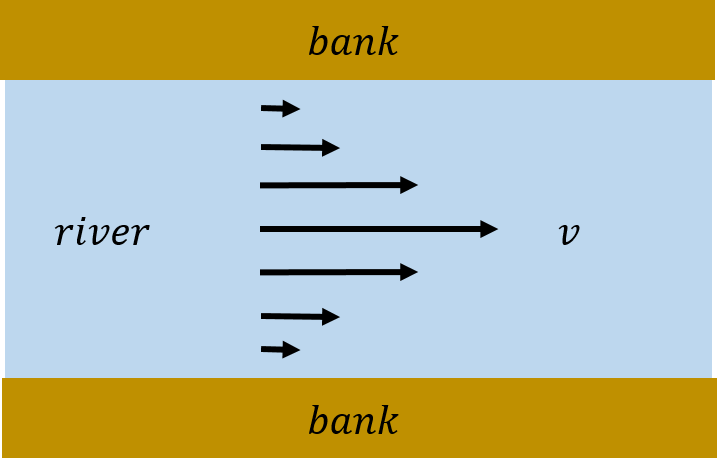
\includegraphics[width=0.4\linewidth]{files/river-96493f15d3659429096014fa3a899881.png}
\caption[]{Water flowing in a river; the water near the banks is almost immobile due to the viscosity of the water.}
\label{fig:fluidmechanics:river}
\end{figure}

One can model the banks of the river as exerting a frictional force on the layer of water that is in contact with the banks. That layer then exerts a frictional force on the next layer closer to the centre of the river, and so on.

One can define a viscosity coefficient, $\eta$, based on measuring the force required to pull a plate past another plate when there is a fluid between the plates. Consider two plates that have an area, $A$, that are a distance $l$ apart, and contain the fluid of interest between them, as illustrated in Figure~\ref{fig:fluidmechanics:viscosity}.

\begin{figure}[!htbp]
\centering
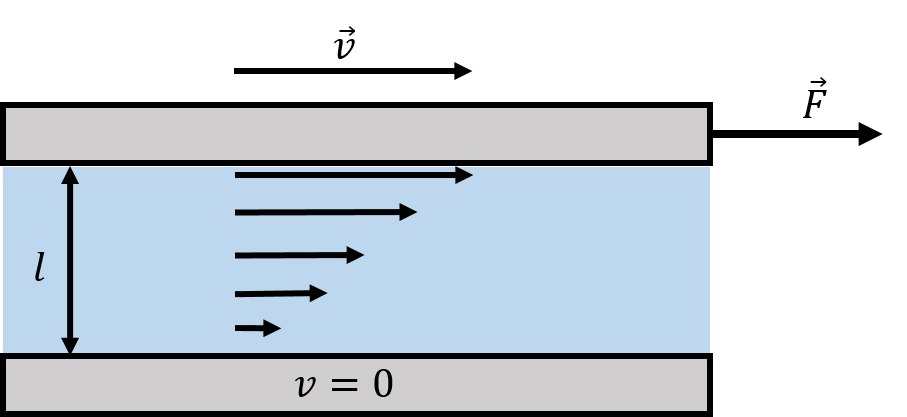
\includegraphics[width=0.5\linewidth]{files/viscosity-a79bba2b6d3a1371a42862b25a925a50.png}
\caption[]{A fluid placed between a moving plate (top) and a fixed plate (bottom) in order to measure the viscosity of the fluid.}
\label{fig:fluidmechanics:viscosity}
\end{figure}

The viscosity of the fluid is defined based on the force that is required to pull the top plate while the bottom plate remains immobile. The layer of fluid directly below the moving plate will move with the plate at a speed, $v$, while the layer of fluid immediately in contact will the stationary plate will also be stationary. Moving one plate will thus lead to a gradient (a change) in the speed of the fluid as a function of the position between the two plates. The magnitude of the force, $\vec F$,  required to move one plate with speed, $v$, was empirically determined to be proportional to the area of the plates, $A$, and the speed, $v$, while being inversely proportional to the distance, $l$, between the two plates:
\begin{equation}
F \propto A\frac{v}{l}
\end{equation}
The constant of proportionality is defined as the viscosity, $\eta$, of the fluid:
\begin{equation}
\boxed{F = \eta A\frac{v}{l}}
\end{equation}
If the viscosity of the fluid is zero, then no force is required to pull the plate. The more viscous the fluid, the more difficult it is to pull the top plate. You can experiment with this by comparing the force required to move a small piece of paper across the top of a puddle of water and across the top of honey.

The presence of viscosity means that any fluid that flows will lose mechanical energy due to internal friction (which will heat up the fluid). Thus, Bernoulli's equation is not correct if the fluid has viscosity, as a fluid cannot flow through a horizontal pipe without a change in pressure to overcome the losses due to friction.

\paragraph{Poiseuille flow}\label{sec:fluidmechanics:poiseuille}

For the flow of an incompressible viscous fluid through a pipe, one can postulate that the flow rate, $Q$, is proportional to the change in pressure, $\Delta P$, across the pipe:
\begin{equation}
Q \propto \Delta P
\end{equation}
where $\Delta P$ is taken as the positive difference between the pressure at either end of the pipe. The fluid flows from high pressure to low pressure. We can introduce a constant of proportionality, $R$, to be the ``resistance of the pipe'', so that we can write:
\begin{equation}
Q = \frac{\Delta P}{R}
\end{equation}
where we wrote the constant of proportionality as $1/R$, so that a larger value of $R$ corresponds to a pipe with a higher resistance to flow. That is, for a given pressure difference, as one increases the resistance of the pipe, one decreases the flow rate through that pipe. The relationship above can be used to empirically determine the resistance of a pipe.

The flow through a pipe with a given resistance will be zero if there is no pressure gradient in the fluid along the pipe. Conversely, if there is no flow of fluid in the pipe, the pressure is the same everywhere in the pipe. We can thus also view a drop in pressure in a pipe to be the result of flow of liquid through the pipe. The pressure cannot drop across a horizontal pipe if there is no flow.

When you close the tap on your kitchen faucet, the pressure inside the faucet is close to the pressure in the main water line that supplies your house. As soon as you open the tap and allow water to flow, the pressure in your faucet drops to atmospheric pressure, and the resulting pressure gradient from the main supply forces water to flow out of the faucet. If you try to plug your kitchen faucet with your thumb and stop the flow of water, you will need to exert a force large enough to overcome the pressure that exists in the main water supply. You will find that it is practically impossible to stop the flow of water with your thumb, as the pressure in the main supply needs to be high enough to overcome the resistance of the pipes and still result in a usable flow of water.

Poiseuille first developed a model for the \textbf{laminar flow of a liquid through a uniform horizontal cylindrical pipe} of length, $L$, with a circular cross-section with radius $r$. He found that the resistance of such a pipe to a fluid of viscosity, $\eta$, is given by:
\begin{equation}
R = \frac{8\eta L}{\pi r^4}
\end{equation}
This makes some intuitive sense, as we expect more resistance (more impedance to flow), if the pipe is longer and if the fluid is more viscous (the resistance is zero if there is no viscosity). We further expect less resistance if the pipe has a larger radius. The resistance found by Poiseuille goes down as the fourth power of the radius. Thus, a pipe that is twice as wide will have a volume flow that is $2^4=16$ times larger because of the reduced resistance.

The laminar flow rate, $Q$, of a viscous fluid through a pipe of length $L$ and radius $R$, when there is a pressure difference $\Delta P$, is given by:
\begin{equation}
\boxed{Q =  \frac{\pi r^4}{8\eta L}\Delta P}
\end{equation}
This is usually referred to as ``Poiseuille's Equation''.

\begin{framed}
\textbf{Checkpoint}\\
Does the flow rate of water out of a garden hose depend on the length of the hose?

\begin{enumerate}
\item No, since the volume of water entering the hose must also exit the hose, it does not matter how long the hose is.
\item Yes, the resistance of the hose depends on its length, so the pressure drop across the hose will change, and so will the flow rate.
\end{enumerate}

\begin{framed}
\textbf{Answer}\\
\begin{enumerate}[resume]
\item
\end{enumerate}
\end{framed}
\end{framed}

\begin{framed}
\textbf{Example 14.8}\\
You are modelling the flow of water for a city. Two houses are connected in parallel to the main water supply, so that water from the main supply flows into either house 1 or house 2, and the flows out of each house then join up again at the main supply. The difference in pressure, $\Delta P$, between the entry and exit point of water is the same for each house, and each house can be modelled as having a net resistance, $R_{1}$ or $R_2$, to the flow of water, as illustrated in Figure~\ref{fig:fluidmechanics:parallel}. If you model the two houses as being the equivalent of a single ``effective'' house with an effective resistance $R$, what is the value of $R$ in terms of $R_1$ and $R_2$?

\begin{figure}[!htbp]
\centering
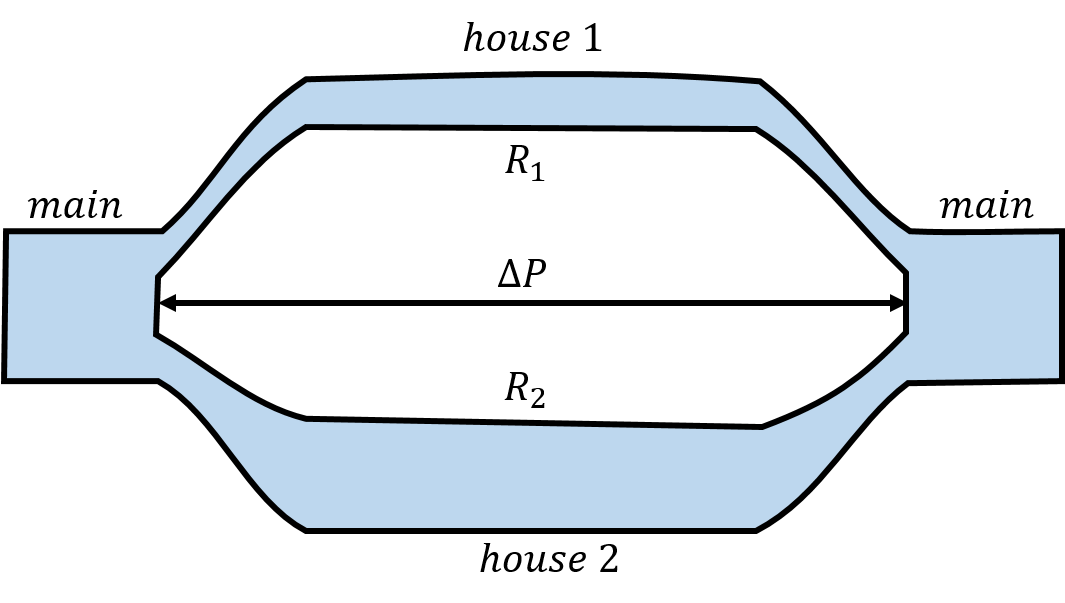
\includegraphics[width=0.7\linewidth]{files/parallel-14e52be1566a62440fcddbe9b5020f5a.png}
\caption[]{Flow of water being separated into two parallel paths that join up again.}
\label{fig:fluidmechanics:parallel}
\end{figure}

\begin{framed}
\textbf{Solution}\\
The water from the main will have to flow through either house 1 or house 2. If the flow rate through the main is $Q$, we require that this be equal to the sum of the flow rates through each house:
\begin{equation}
Q = Q_1 + Q_2
\end{equation}
The flow through each house is related to the pressure difference, $\Delta P$, across each house (which is the same), as well as the resistance of that house:
\begin{equation}
Q_1 &= \frac{\Delta P}{R_1}\\
Q_2 &= \frac{\Delta P}{R_2}
\end{equation}
The total flow rate is thus:
\begin{equation}
Q = Q_1 + Q_2&=\frac{\Delta P}{R_1}+\frac{\Delta P}{R_2}\\
&=\Delta P \left(\frac{1}{R_1}+\frac{1}{R2}\right)
\end{equation}
We can write this as the flow through an effective resistance, $R$, with a pressure difference $\Delta P$:
\begin{equation}
Q &= \frac{\Delta P}{R}\\
\therefore R&= \frac{1}{\frac{1}{R_1}+\frac{1}{R2}}
\end{equation}
\textbf{Discussion:} By requiring that the sum of the flows of water through the houses be the same as the flow rate through the main pipe, we were able to model the two houses as a single effective house with resistance $R$. You may notice that this is the same relation as the equivalent resistance for two electrical resistors combined in parallel. This is because the flow of electrical current in a resistor can be modelled using similar tools to those required for modelling the flow of a viscous fluid in a pipe.
\end{framed}
\end{framed}

\subsubsection{Summary}

The pressure from a force, $\vec F$, exerted over a surface with area, $A$, is a scalar quantity defined as:
\begin{equation}
P = \frac{F_\perp}{A}
\end{equation}
where $F_\perp$ is the component of the force perpendicular to the surface.

If a force is exerted on the particles in a fluid (e.g. gravity), a pressure will exist everywhere in the fluid. If the fluid is placed in a container, that pressure leads to an external force on all surfaces of the container.

If two fluids at different pressures exist on either side of an interface/object, the net force on that interface/object from the pressures of the fluids will be proportional to the difference in pressure of the fluids on either side.

A fluid is in hydrostatic equilibrium if the sum of the forces on any fluid element is zero. In the presence of gravity, this always leads to a vertical pressure gradient
\begin{equation}
\frac{dP}{dy}=-\rho g
\end{equation}
where $\rho$ is the density of the fluid, $g$ is the magnitude of the Earth's gravitational field, and the $y$ axis is positive upwards.

If the fluid is incompressible, then the difference in pressure between two points at heights $y_1$ and $y_2$ is given by:
\begin{equation}
P(y_2)-P(y_1) =-\rho g (y_2-y_1)
\end{equation}
Pascal's Principle states that if an external pressure, $P$, is applied to one location in a fluid, then the pressure everywhere in the fluid increases by $P$.

If an object is immersed in a fluid, it will experience a force of buoyancy that is in the opposite direction to the gravitational field in that fluid. The magnitude of the buoyancy force is given by Archimedes' Principle:
\begin{equation}
F_B = \rho Vg
\end{equation}
where, $\rho$, is the density of the fluid and, $V$, is the volume of the fluid displaced by the object (i.e. the volume of the part of the object that is immersed in the fluid).

We can distinguish between laminar and turbulent flow of fluids. In laminar flow, individual particles in the fluid follow well-defined streamlines. In turbulent flow, individual particle follow complicated paths that usually involve Eddy currents. In general, it is much easier to model the laminar flow of fluids.

The equation of continuity states that the mass flow rate of a fluid through a closed system must be the same everywhere in the system (no fluid can appear or disappear). For laminar flow of a fluid with density, $\rho$, flowing at speed, $v$, through a pipe with cross section, $A$, the mass flow rate is a constant:
\begin{equation}
\rho A v= \text{constant}
\end{equation}
A fluid is said to be incompressible if it has constant density. For a fluid of constant density, the volume flow rate, $Q$, must be constant everywhere in a closed system:
\begin{equation}
Q = Av = \text{constant}
\end{equation}
Bernoulli's Principle, which is based on the conservation of mechanical energy, states that the following quantity is a constant:
\begin{equation}
P + \frac{1}{2}\rho v^2 + \rho g y= \text{constant}
\end{equation}
for the laminar flow of a fluid with no viscosity. $P$ is the internal pressure of the fluid, $v$ its speed, and $y$ the height of the fluid relative to a fixed coordinate system. In particular, Bernoulli's Principle implies that, for a constant height, the internal pressure of a fluid must decrease if its speed increases.

Viscosity, $\eta$, for the laminar flow of a fluid can be modelled as the result of the internal friction force between layers of the fluid. Because of viscosity, a fluid cannot flow in a horizontal pipe unless there is a difference in pressure across the pipe. Similarly, there will be no horizontal pressure gradient through a fluid unless the fluid is flowing. In general, the volume flow rate, $Q$, of an incompressible fluid through a pipe with resistance, $R$, is given by:
\begin{equation}
Q = \frac{\Delta P}{R}
\end{equation}
For the laminar flow of a fluid with viscosity, $\eta$, through a horizontal cylindrical pipe of length, $L$, and radius, $r$, the flow rate is given by Poiseuille's equation:
\begin{equation}
Q =  \frac{\pi r^4}{8\eta L}\Delta P
\end{equation}

\begin{framed}
\textbf{Important Equations}\\
\textbf{In the presence of gravity:}
\begin{equation}
\frac{dP}{dy}&=-\rho g\\
P(y_2)-P(y_1)&=-\rho g(y_2-y_1)\\
F_B&=\rho Vg
\end{equation}
\textbf{Equation of continuity:}
\begin{equation}
\rho Av&=\textrm{constant}\\
Q&=Av=\textrm{constant}\quad \textrm{(if incompressible)}
\end{equation}

\textbf{Bernoulli:}
\begin{equation}
P+\frac{1}{2}\rho v^2+\rho gy=\textrm{constant}
\end{equation}
\textbf{Viscosity:}
\begin{equation}
Q&=\frac{\Delta P}{R}\\
Q&= \frac{\pi r^4}{8\eta L}\Delta P \quad \textrm{(Poiseuille)}
\end{equation}
\end{framed}

\begin{framed}
\textbf{Important Definitions}\\
\begin{itemize}
\item \textbf{Pressure:} A measurement of force per unit area. SI units: [ ${\rm Pa}$]. Common variable(s): $P$.
\item \textbf{Viscosity:} A measurement of a fluid's resistance to flow. SI units: [ ${\rm Pa\cdot s}$]. Common variable(s): $\eta$.
\item \textbf{Flow rate:} Measurement of a fluid's motion, in volume per unit time. SI units: [ ${\rm m^3s^{ -1}}$]. Common variable(s): $Q$.
\end{itemize}
\end{framed}

\subsubsection{Thinking about the material}

\begin{framed}
\textbf{Reflect and research}\\
\begin{itemize}
\item Does atmospheric pressure increase or decrease when the weather is nice? How come?
\item How does water move from the roots of a tree to the top, for a very tall tree?
\item When did Bernoulli describe the motion of fluids?
\item Where did Bernoulli come from?
\end{itemize}
\end{framed}

\begin{framed}
\textbf{To try at home}\\
\begin{itemize}
\item Place your hand in a plastic bag, and immerse your hand with the bag in water. The deeper the column of water, the better. Describe what you feel on your hand in terms of the direction of the force exerted by the water pressure.
\item If you assume that the water that comes out of your bathroom faucet is gravity-fed from a water tank, determine the height of the corresponding water tower relative to your bathroom faucet. Measure the flow rate of water from the faucet to determine the height and discuss whether it makes sense.
\item Try plugging the faucet in your bathroom tap with your thumb. Are you able to completely prevent water from coming out when the tap is open? Estimate the pressure of the water in the pipes leading to your bathroom faucet.
\item In your house/building, measure the flow rate between similar faucets at different heights, and compare with what one would expect from the model from Example~14.7.
\end{itemize}
\end{framed}

\begin{framed}
\textbf{To try in the lab}\\
\begin{itemize}
\item Propose an experiment to build a barometer and track the changes in atmospheric pressure as a function of time, and to compare your measurements to those from a weather station.
\item Propose an experiment to characterize how liquid flows in a sponge. Is there a maximum height to which a sponge can draw liquid? How is energy conserved if water is drawn upwards in a sponge?
\item Propose an experiment to measure the resistance of a pipe to the flow of water and compare with the result expected from Poiseuille's equation.
\item Propose an experiment to determiner the viscosity of maple syrup.
\item Propose an experient to model the water flow in the sections of a cascading fountain.
\item Investigate the flow of water in a spinning bowl.
\item Investigate and model how the pressure in a balloon changes as the balloon increases in volume.
\item Investigate and model the surface tension of water.
\item Design and build a blood pressure monitor using a manometer.
\end{itemize}
\end{framed}

\subsubsection{Sample problems and solutions}

\paragraph{Problems}

\begin{framed}
\textbf{Problem 14.1}\\
A man and a woman, Rebecca (57 \{{\textbackslash}rm kg\}) and Ryan (63 \{{\textbackslash}rm kg\}), are on a cruise when their ship tragically sinks. They are thrust into the freezing cold ocean. They see a large wooden door floating on the surface of the water, and wonder if they could both survive if they both lay on top of the door. They estimate that the door measures about $2 {\rm m}\times1 {\rm m}\times0.12 {\rm m}$. The density of salt water is $\rho_w=1027 {\rm kg/m^3}$.

\begin{figure}[!htbp]
\centering
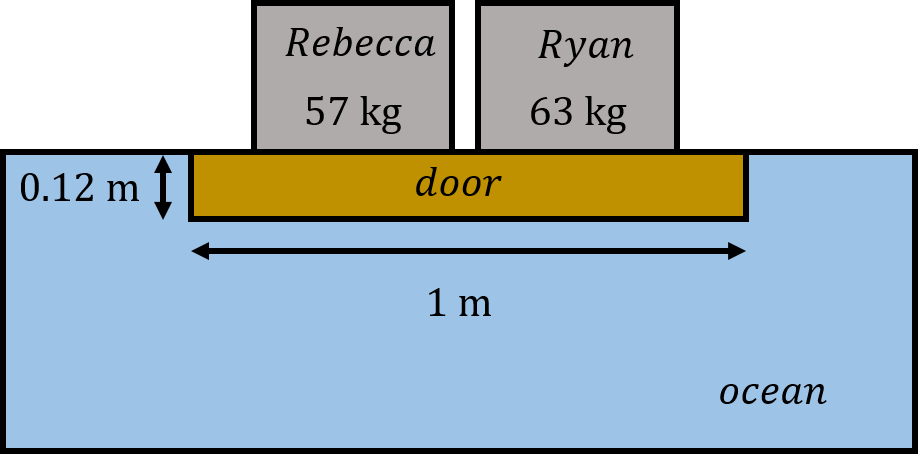
\includegraphics[width=0.6\linewidth]{files/notthetitanic-35c349e53d4639c24b4cf5780a40df06.png}
\caption[]{Rebecca and Ryan wonder if they can stay above water if they get on top of a floating door.}
\label{fig:fluidmechanics:notthetitanic}
\end{figure}

\begin{itemize}
\item a. What does the density of the wood have to be in order for Rebecca and Ryan to stay above the surface of the water? (see Figure~\ref{fig:fluidmechanics:notthetitanic})
\item b. If the door is made of oak ($\rho_d=750 {\rm kg/m^3}$), will they survive? Can one of them survive?
\end{itemize}
\end{framed}

\begin{framed}
\textbf{Problem 14.2}\\
A doctor prescribes an IV drip to a dehydrated patient. She asks a nurse, Rob, to administer $2 {\rm l}$ of saline solution ($\eta=1.0\times 10^{ -3} {\rm Pa\cdot s}$, $\rho=997 {\rm kg/m^3}$) to the patient over 2 hours. An IV drip works by inserting a needle into a vein in a patient's arm. The needle is connected to an IV bag by a tube (Figure~\ref{fig:fluidmechanics:ivneedle}). Lily uses a needle that has a diameter of 0.60 \{{\textbackslash}rm mm\} and a length of 32 \{{\textbackslash}rm mm\}. The blood pressure in the patient's veins is $80 {\rm mm Hg}$ above atmospheric pressure. Note: $1 {\rm mm Hg}\approx 133 {\rm Pa}$

\begin{figure}[!htbp]
\centering
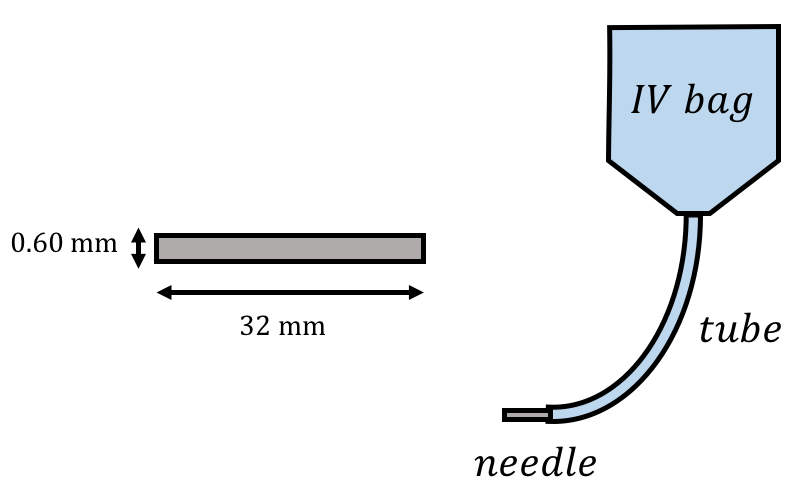
\includegraphics[width=0.6\linewidth]{files/ivneedle-b6d18068c82e3e182f801489e01b81ca.png}
\caption[]{Left: A cylindrical IV needle. Right: The IV needle connected to an IV bag by a tube. The free end of the needle goes into the patient's vein.}
\label{fig:fluidmechanics:ivneedle}
\end{figure}

\begin{itemize}
\item a. What must the pressure be at the entrance of the needle (the side connected to the saline, not the patient)? Assume that the needle is essentially horizontal and that the diameter of the tube from the IV bag is large enough so that resistance in the vertical tube is negligible. Write your answer in Pascals above atmospheric pressure.
\item b. How high above the patient's arm should Lily put the IV bag?
\end{itemize}
\end{framed}

\paragraph{Solutions}

\begin{framed}
\textbf{Solution 14.1}\\
\begin{itemize}
\item a. The forces acting on the door are the force of buoyancy, the door's weight, and the weights of Rebecca and Ryan, as shown in Figure~\ref{fig:fluidmechanics:notthetitanic_fbd}.
\end{itemize}

\begin{figure}[!htbp]
\centering
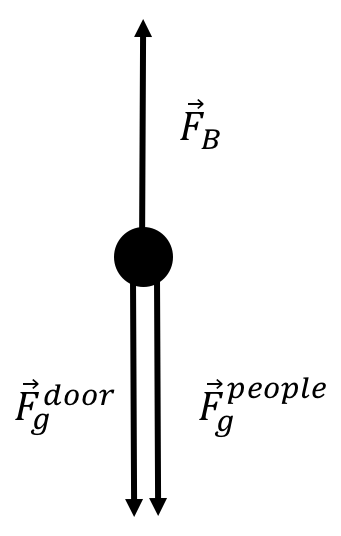
\includegraphics[width=0.2\linewidth]{files/notthetitanic_fbd-5bca048002d3a8722feb70324b7a36ad.png}
\caption[]{The forces acting on the door when Rebecca and Ryan are on top of it.}
\label{fig:fluidmechanics:notthetitanic_fbd}
\end{figure}

We can combine the weight of the door and the weight of the people into the total weight, $F_g$. We choose the $y$ axis to be positive upwards. The sum of the forces on the door in the $y$ direction is given by:
\begin{equation}
\sum F_y = F_B- F_g
\end{equation}
For the door to float, the net force on the door must be greater than or equal to zero. We want to find the minimum buoyant force for them to float, so we set the net force equal to zero:
\begin{equation}
F_g&=F_B\\
(m_R+m_r+m_d)g&=\rho_wV_wg\\
m_R+m_r+m_d&=\rho_wV_w
\end{equation}
where the weight includes the mass of Rebecca ($m_R$), Ryan ($m_r$) and the door ($m_d$). We added the subscript $W$ to the right side of the equation to remind ourselves that the buoyant force depends on the density and volume \textbf{of the displaced water}. We want to find the maximum density of the wood in order for Rebcca and Ryan to stay above the water's surface. This means that the maximum volume of water that can be displaced is the volume of the door, $V_w=V_d$ (so that the surface of the door is level with the surface of the water, as in Figure~\ref{fig:fluidmechanics:notthetitanic}). We can rewrite the mass of the door in terms of its volume and density, and apply our condition that $V_w=V_d$ :
\begin{equation}
m_R+m_r+\rho_dV_d&=\rho_wV_d\\
\rho_d&=\frac{\rho_wV_d-m_R-m_r}{V_d}
\end{equation}
A quick calculation tells us that the volume of the door is $(2 {\rm m})(1 {\rm m})(0.12 {\rm m})=0.24 {\rm m^3}$. We can now calculate the desired density of the wood:
\begin{equation}
\rho_d&=\frac{\rho_wV_d-m_R-m_r}{V_d}\\
\rho_d&=\frac{(1027 {\rm kg/m^3})(0.24 {\rm m^3})-57 {\rm kg}-63 {\rm kg}}{0.24 {\rm m^3}}\\
\rho_d&=527 {\rm kg/m^3}
\end{equation}
The maximum density of the wood that would allow them to both float is $527 {\rm kg/m^3}$. Balsa wood has a density that is about $150 {\rm kg/m^3}$, so would allow them to survive. However, it is unlikely that a random floating door is made of balsa wood (although one would choose lighter materials when constructing a ship).

\begin{itemize}
\item b. No, they could not both stay on the door because the density of oak is greater than the maximum density of $527 {\rm kg/m^3}$. We can find the amount of mass that can be added to the door ($m_A$) in order for the person on it to stay above water:
\end{itemize}
\begin{equation}
F_g&=F_B\\
(m_A+m_d)g&=\rho_wV_wg\\
m_A+\rho_dV_d&=\rho_wV_w\\
m_A+\rho_dV_d&=\rho_wV_d\\
m_A&=V_d(\rho_w-\rho_d)
\end{equation}
where we again used the condition that $V_w=V_d$. We can plug in the appropriate values and solve:
\begin{equation}
m_A&=V_d(\rho_w-\rho_d)\\
m_A&=(0.24 {\rm m^3})(1027 {\rm kg/m^3}-750 {\rm kg/m^3})\\
m_A&=66 {\rm kg}
\end{equation}
The door can support an additional mass of $66 {\rm kg}$, so either Rebecca or Ryan can survive if the other does not get on the door.
\end{framed}

\begin{framed}
\textbf{Solution 14.2}\\
\begin{itemize}
\item a. Given that the pressure in the patient's veins is $80 {\rm mm Hg}$ above atmospheric pressure, we want to find the pressure required at the other end of the needle so that we get the desired flow rate through the needle. We model the needle as a horizontal cylindrical pipe and assume that the saline solution exhibits laminar flow. We can therefore use Poiseuille's equation:
\end{itemize}
\begin{equation}
Q=\frac{\pi r^4}{8\eta L}(P_1-P_2)
\end{equation}
We let $P_1$ be the pressure where the needle connects to the tube. Solving for $P_1$ gives:
\begin{equation}
P_1=Q\frac{8\eta L}{\pi r^4}+P_2\\
\end{equation}
The pressure at the exit of the needle, $P_2$, is just the blood pressure ($80 {\rm mm Hg} + 1 {\rm atm}$). The radius of the needle is $0.60 {\rm mm}/2=0.30 {\rm mm}$. The flow rate has to be in units of ${\rm m^3/s}$. The flow rate in the appropriate units is thus:
\begin{equation}
Q=\frac{2 {\rm l}}{2 {\rm hr}}\cdot \frac{1 {\rm hr}}{3600 {\rm s}}\cdot \frac{0.001 {\rm m^3}}{1 {\rm l}}=2.8\times 10^{-7} {\rm m^3/s}
\end{equation}
Using our values, we can calculate $P_1$:
\begin{equation}
P_1 &= (2.8\times 10^{-7} {\rm m^3/s})\frac{8(1.0\times 10^{3} {\rm Pa\cdot s}) (0.032 {\rm m})}{\pi (3\times 10^{-4} {\rm m})^4}+80 {\rm mm Hg}\cdot \frac{133 {\rm Pa}}{1 {\rm mm Hg}}+1 {\rm atm}\\
P_1 &= 2817 {\rm Pa}+10640 {\rm Pa}+1 {\rm atm}\\
\therefore P_2 &= 13457 {\rm Pa} \quad \textrm{above atmospheric pressure}
\end{equation}
Note that, in the first line, we converted $80 {\rm mm Hg}$ into Pascals.

\begin{itemize}
\item b. We can  easily determine the height of the IV bag that is required to give the desired pressure. We choose a coordinate system with a $y$ axis that is vertical (positive upwards) with the origin at the location of the needle (Figure~\ref{fig:fluidmechanics:ivneedleheight}).
\end{itemize}

\begin{figure}[!htbp]
\centering
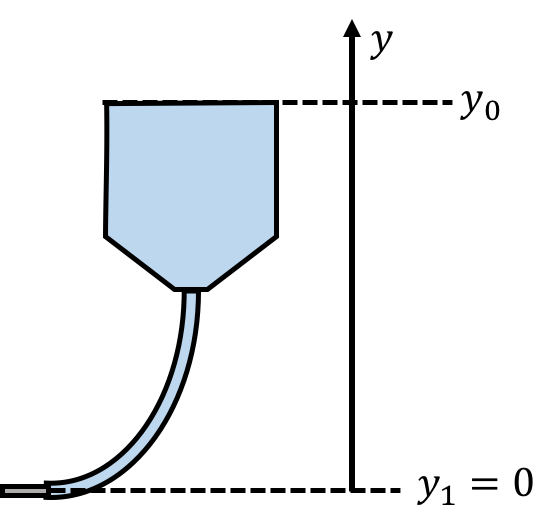
\includegraphics[width=0.3\linewidth]{files/ivneedleheight-91f4b9fd11e610882256154a027e4588.png}
\caption[]{The needle is at height 0 and the top of the fluid in the IV bag is at $y_0$.}
\label{fig:fluidmechanics:ivneedleheight}
\end{figure}

At the top of the solution in the IV bag, $y_0$, the solution has a speed of zero and is at atmospheric pressure, $P_0=1 {\rm atm}$. The velocity at the needle is 0, and the pressure is $13457 {\rm Pa}+1 {\rm atm}$. Bernoulli's principle states:
\begin{equation}
P_0+\frac{1}{2}\rho v_0^2+\rho gy_0=P_1+\frac{1}{2}\rho v_1^2+\rho gy_1\\
\end{equation}
Using our values to solve for $y_0$, we get:
\begin{equation}
P_0+\rho gy_0&=P_1\\
y_0&=\frac{P_1-P_0}{\rho g}\\
y_0&=\frac{13457 {\rm Pa}+1 {\rm atm}-1 {\rm atm}}{(997 {\rm kg/m^3})(9.8 {\rm m/s^2})}\\
y_0&=\frac{13457 {\rm Pa}}{(997 {\rm kg/m^3})(9.8 {\rm m/s^2})}\\
y_0&=1.4 {\rm m}
\end{equation}
Therefore, the IV bag should be placed $1.4 {\rm m}$ above the patient's arm.
\end{framed}